\chapter{Experiments}
\label{chapter_experiments}
The measurement process to identify the body parameters starts after a subject is recognized,
identified and calibrated for tracking. Following the parameter estimation, the virtual avatar and cloth are created and the 
simulation starts.

Experiments are performed on a high-end PC with Intel i7-2600 and NVIDIA GeForce GTX560Ti. The total time for the measurement of body parameters and resizing the cloth does not exceed 1.005 seconds. Considering the time for acquiring 30 frames of input from the depth sensor is 1.0 second, it is safe to say that the measurement algorithm does not introduce any delays for a real time application because it needs to run only once at the beginning of the simulation. The actual simulation runs at 600 fps on $1920 \times 1080$ resolution. The body sizes are estimated with error rates less than 4\%, which is sufficient for the realism of the simulation and determining the appropriate apparel size.

Table~\ref{tbl:body_results} presents the measurements of the body dimensions, as well as the errors and standard deviations of the measurements in 30 frames for three subjects. Our results are compared with the results from~\cite{Giovanni2012} and \cite{Samejima2012}, which are also real-time applications, in Table~\ref{tbl:performance_compare}.

\singlespacing

\begin{table}
\begin{center}
\begin{tabular}{|c|c|c|c|c|c|c|c|c|}
\hline
  & \multicolumn{4}{c|}{\textbf{Shoulder Width (cm)}} & \multicolumn{4}{c|}{\textbf{Body Height (cm)}} \\ \hline
  \rotatebox{90}{Subject } & \rotatebox{90}{Real } & \rotatebox{90}{Estimated } & \rotatebox{90}{Error (\%)} & \rotatebox{90}{Deviation } & \rotatebox{90}{Real } & \rotatebox{90}{Estimated } & \rotatebox{90}{Error (\%)} & \rotatebox{90}{Deviation } \\ \hline
 1 & 43 & 43.6 & 1.0 & 7.8 & 172 & 170.8 & 0.6 & 2.5  \\ \hline
 2 & 46 & 44.3 & 3.0 & 8.5 & 176 & 172.1 & 2.0 & 1.4  \\ \hline
 3 & 51 & 48.8 & 4.0 & 12.1 & 176 & 174.0 & 1.0 & 6.6  \\ \hline
 4 & 48 & 50.0 & 4.0 & 2.5 & 188 & 191.0 & 1.5 & 7.1  \\ \hline
 5 & 44 & 42.6 & 3.0 & 4.2 & 178 & 175.8 & 1.2 & 3.1  \\ \hline
\end{tabular}
\end{center}
\caption{Performance figures for five different subjects.}
\label{tbl:body_results}
\end{table} 



\begin{table}
\begin{center}
\begin{tabular}{|l|c|c|c|c|} 
\hline 
  & \rotatebox{90}{\parbox[c]{2.95cm}{\mbox{Error Average} \mbox{\hspace{0.7cm}(\%)}}} & \rotatebox{90}{\parbox[c]{2.95cm}{\mbox{Error Deviation} \mbox{\hspace{0.7cm}(\%)}}} & \rotatebox{90}{Duration} & \rotatebox{90}{Estimation} \\ \hline
  Our Approach & 2.13  & 1.20   & 1.00 & Fixed \\ \hline 
  Giovanni et al.~\cite{Giovanni2012}  & 4.00  & 3.00  & 1.00 & None \\ \hline
  Samejima et al.~\cite{Samejima2012}  & 6.72  & 4.68  & n/a & PCA \\ \hline
\end{tabular}
\end{center}  
\caption{Performance comparison with \cite{Giovanni2012} and \cite{Samejima2012} regarding height measurements.}
\label{tbl:performance_compare}
\end{table}

\doublespacing 

For the collision spheres, the quality of the results can be assessed by the smoothness of the collision simulation, as seen in Figure \ref{fig:system}. Throughout the simulation, unnatural intersections between the cloth and the avatar never take place, while the cloth appears to rest on the skin naturally, without space between the two meshes. Figure~\ref{fig:examples} shows examples of three garments on a model with different postures generated with our implementation. 

\begin{figure}[htbp]
	\begin{center} 
			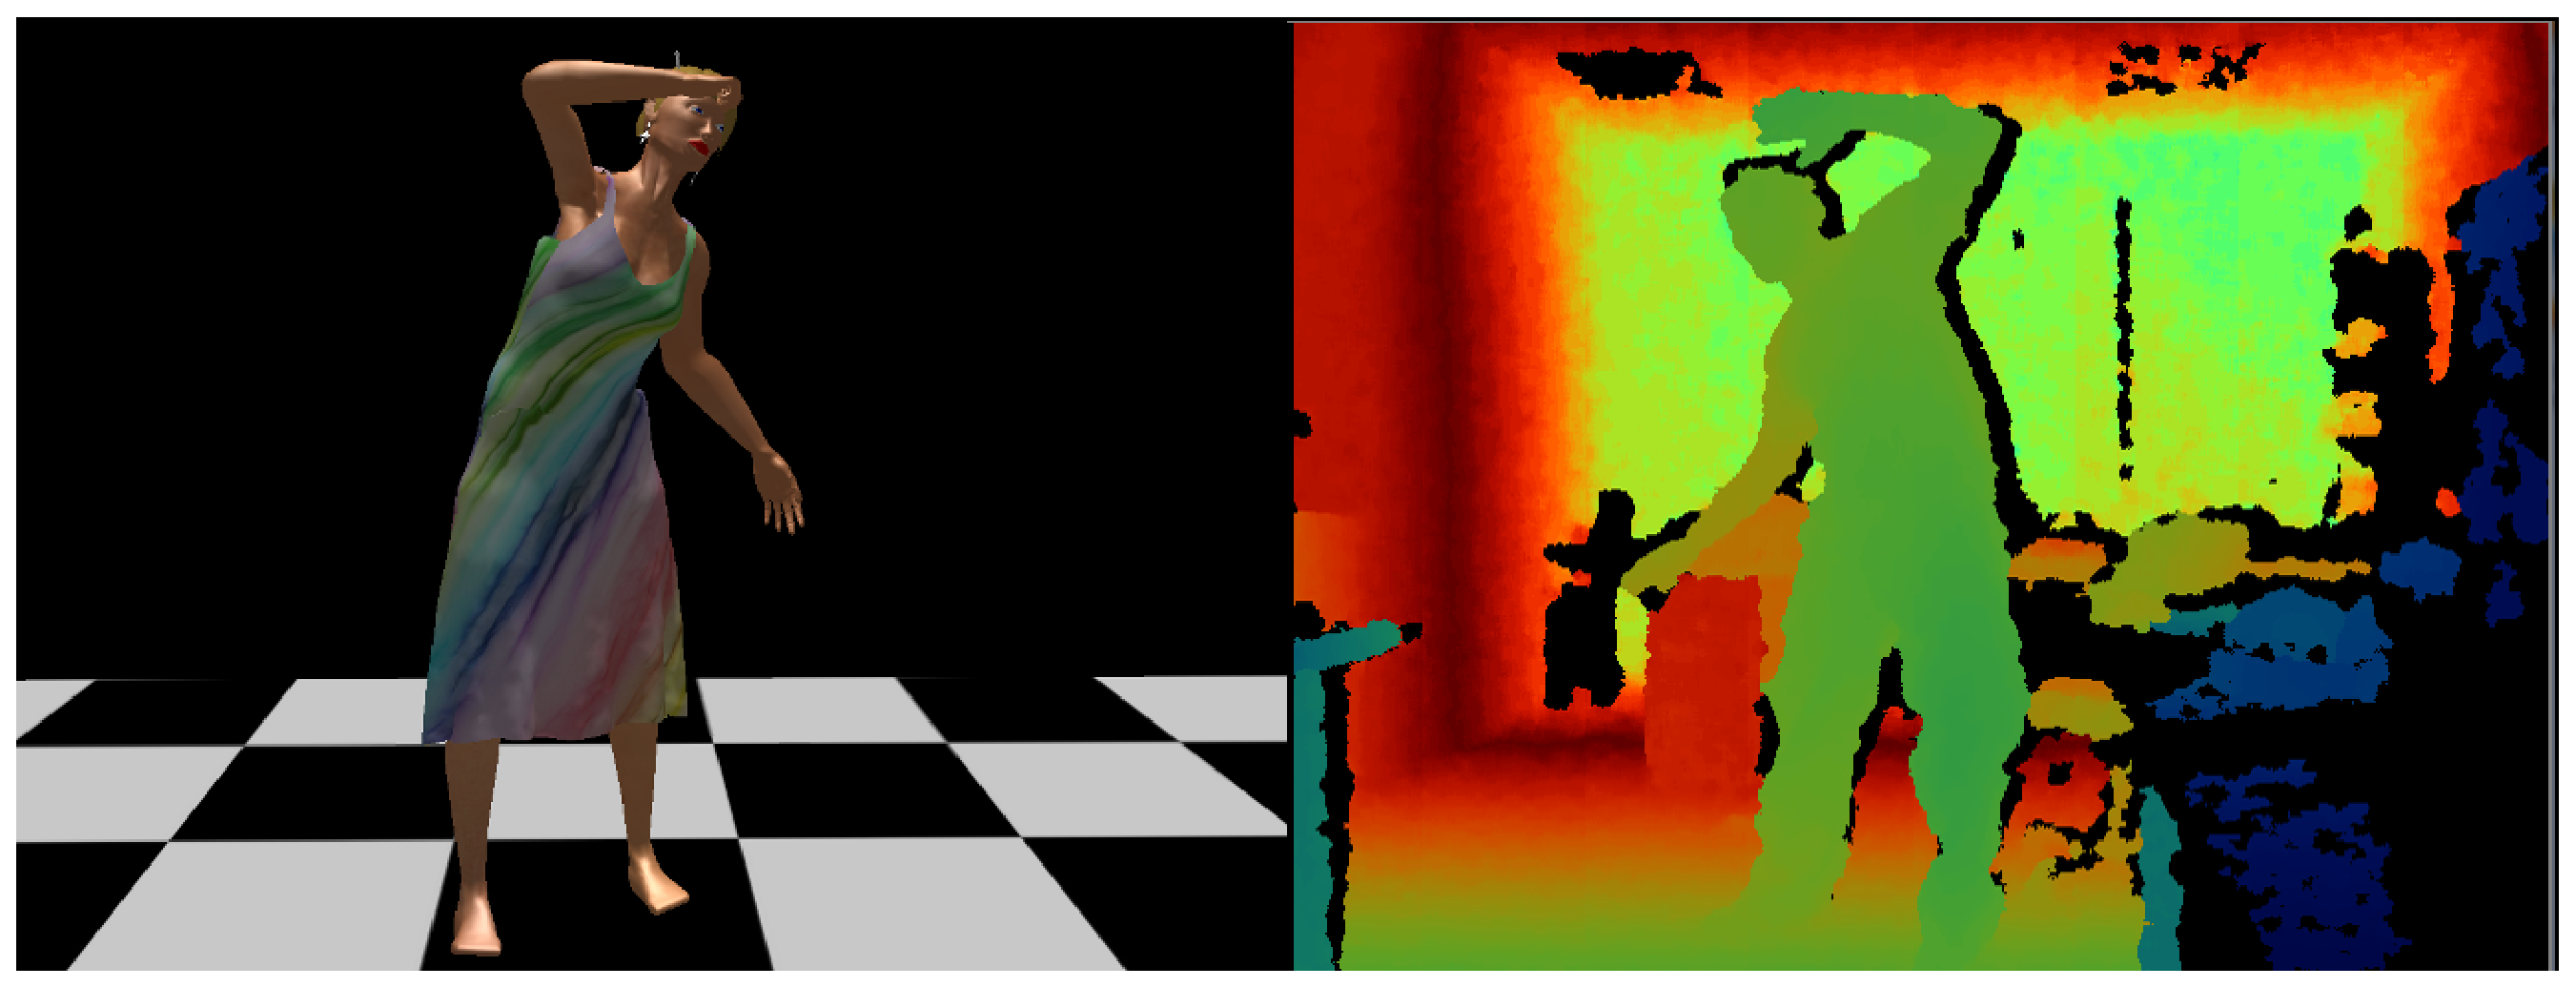
\includegraphics[width=1.00\textwidth]{./figures/scshot.eps}
	\end{center}
	\caption{An example depth map data and the corresponding posture of the subject with a virtual cloth on it.}
	\label{fig:system}
\end{figure}
 
 \begin{figure}[htbp] 
	\centerline{
	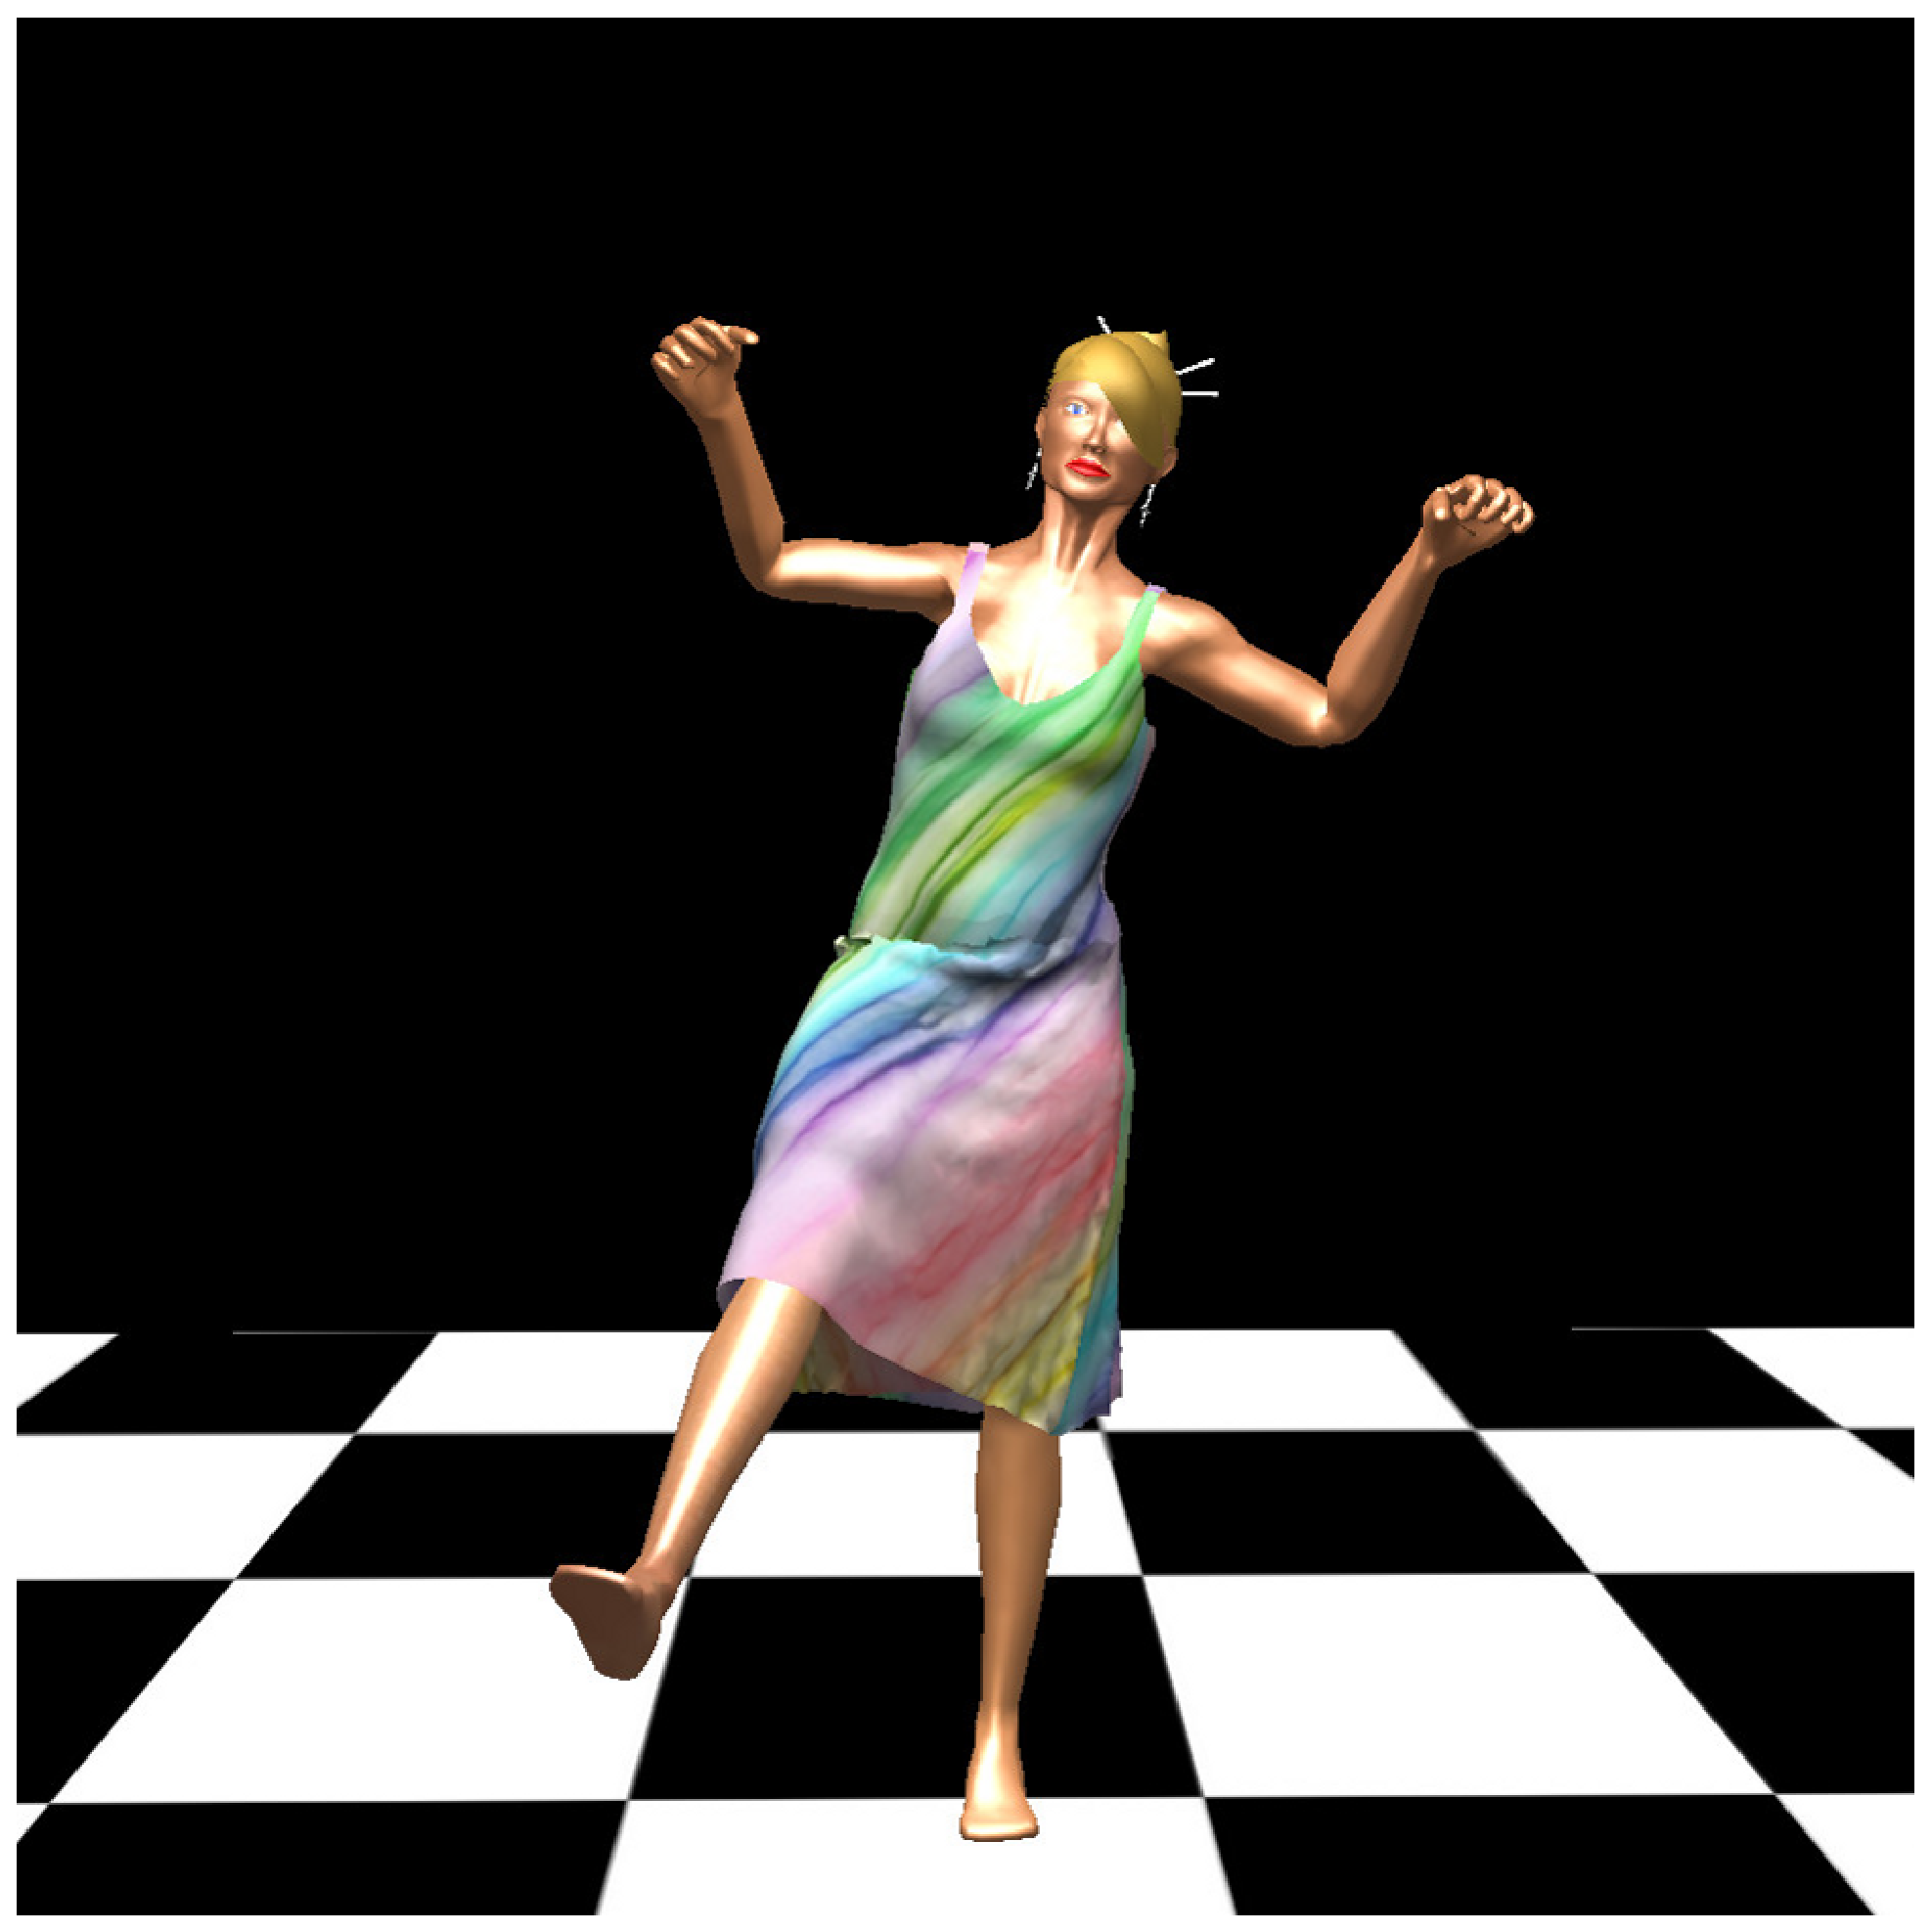
\includegraphics[width=0.250\textwidth]{./figures/sundress1.eps}
	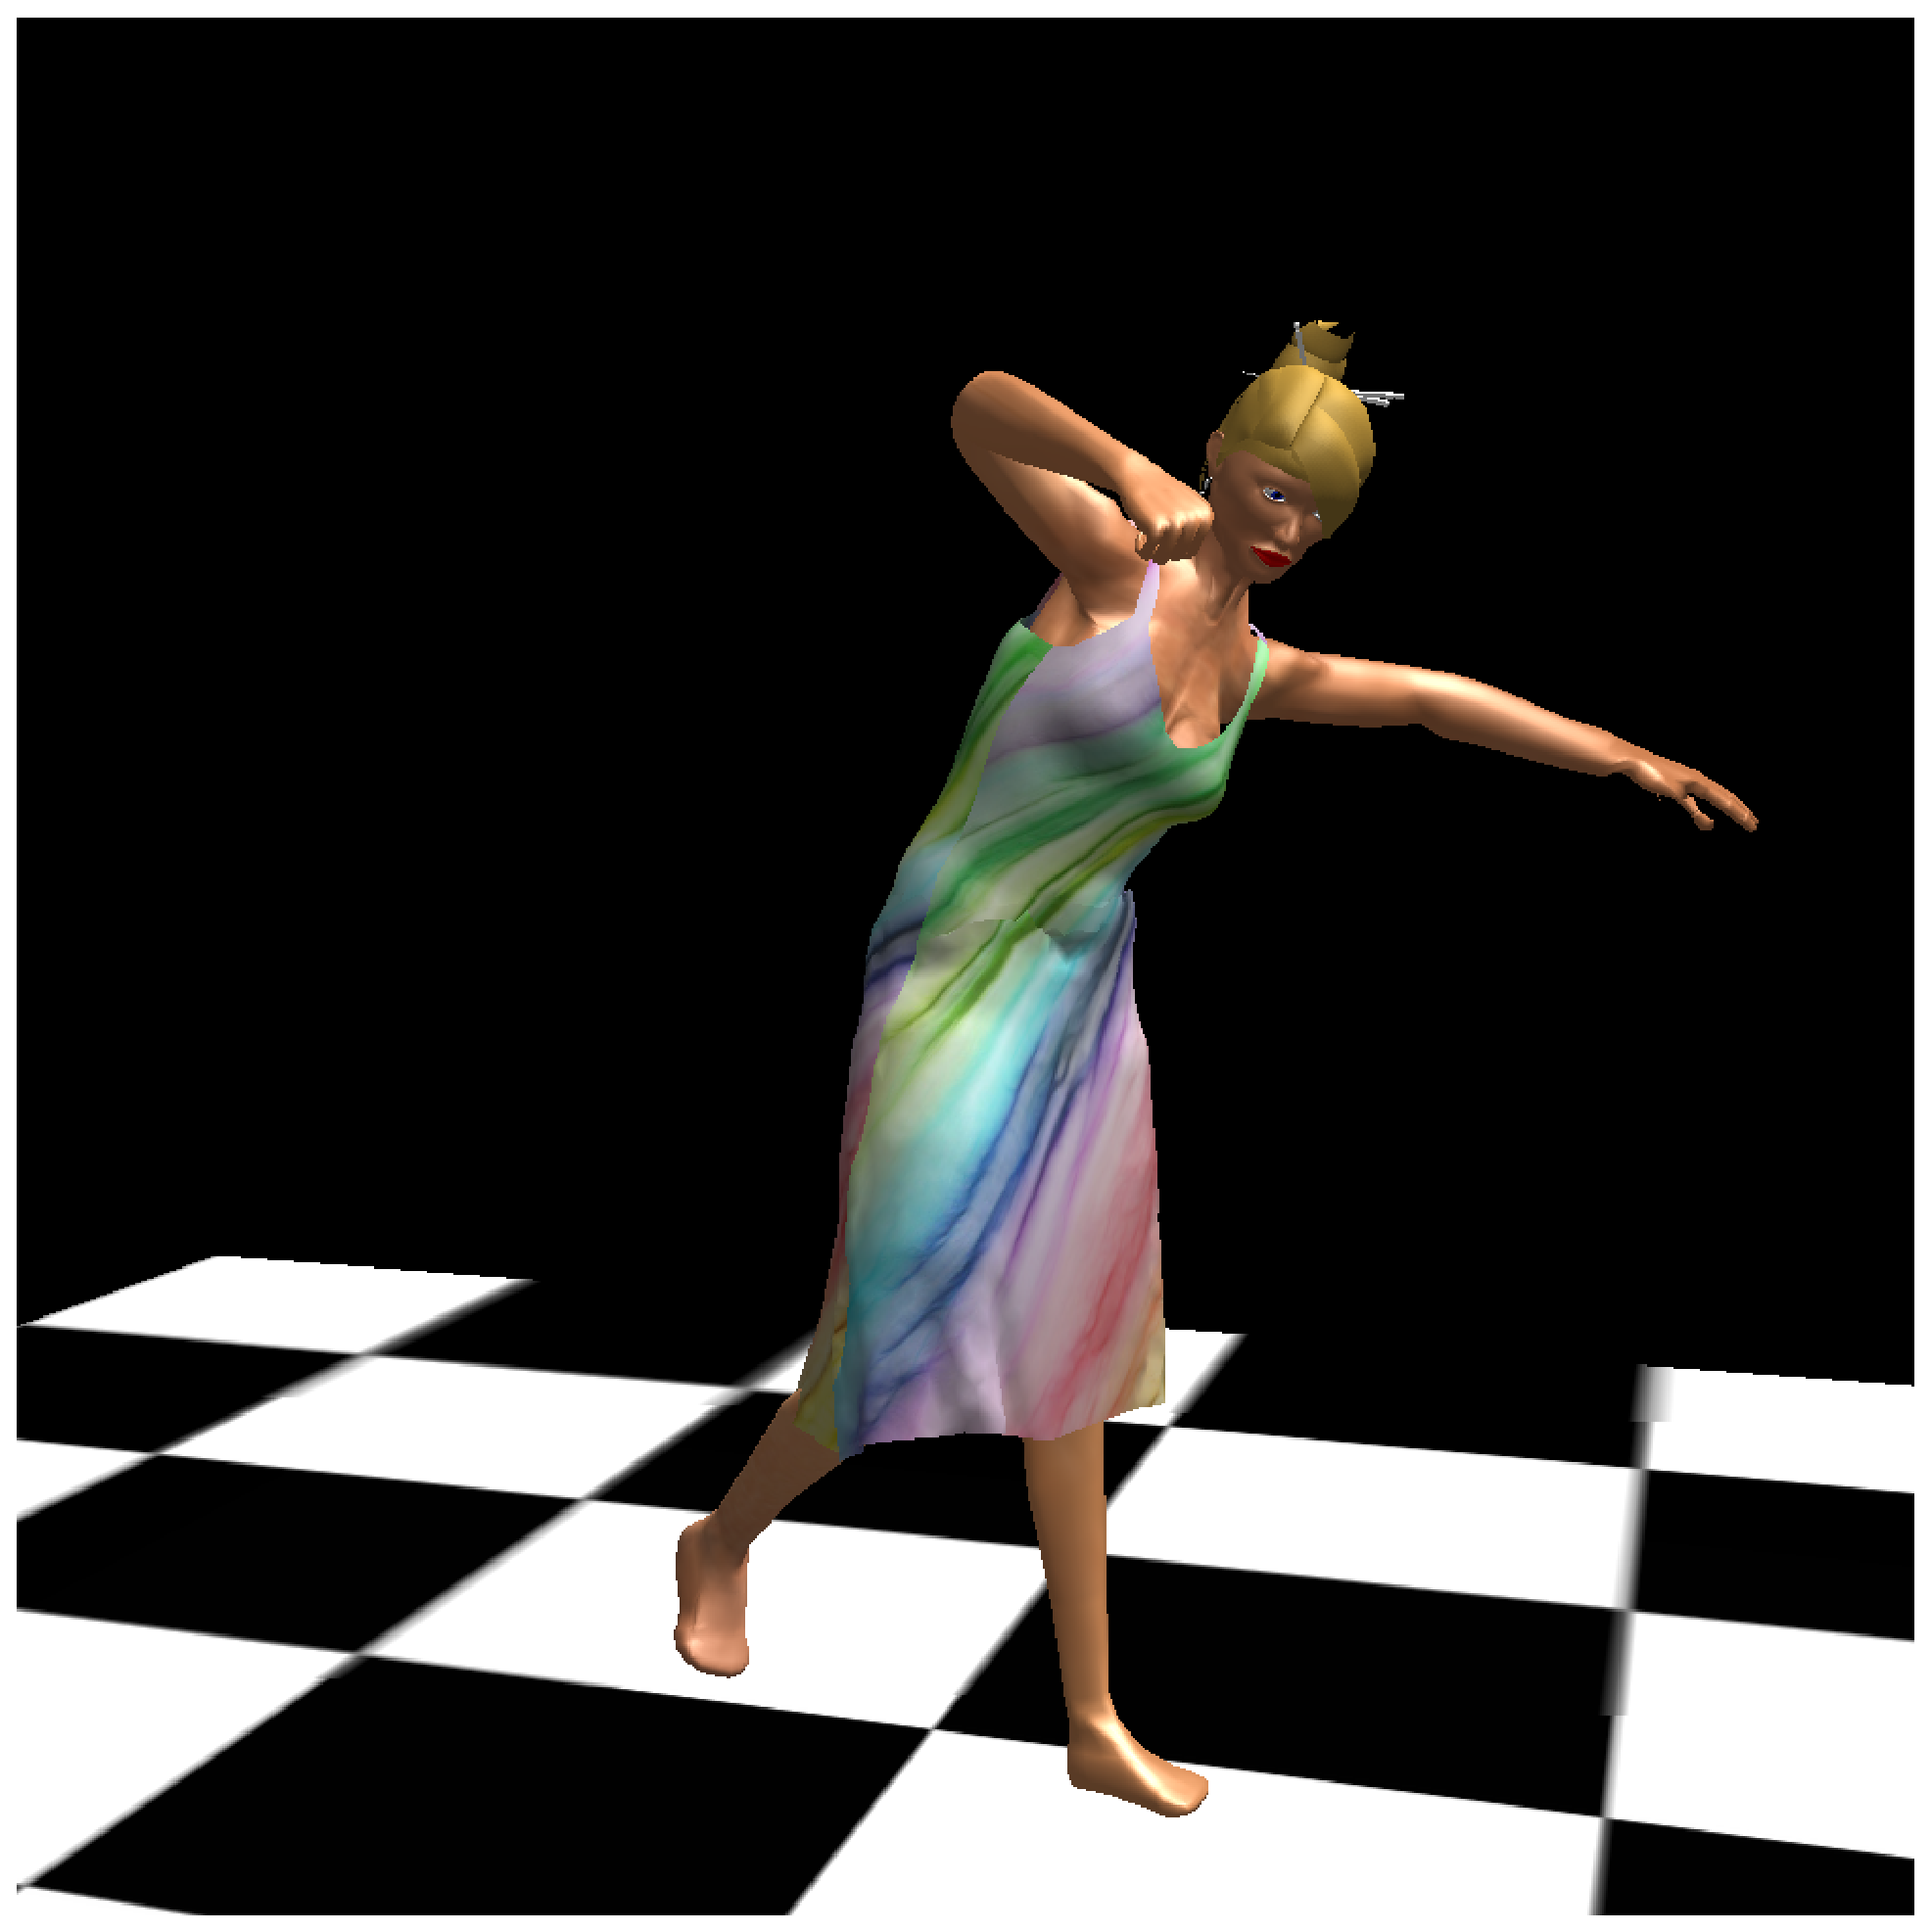
\includegraphics[width=0.250\textwidth]{./figures/sundress2.eps}
	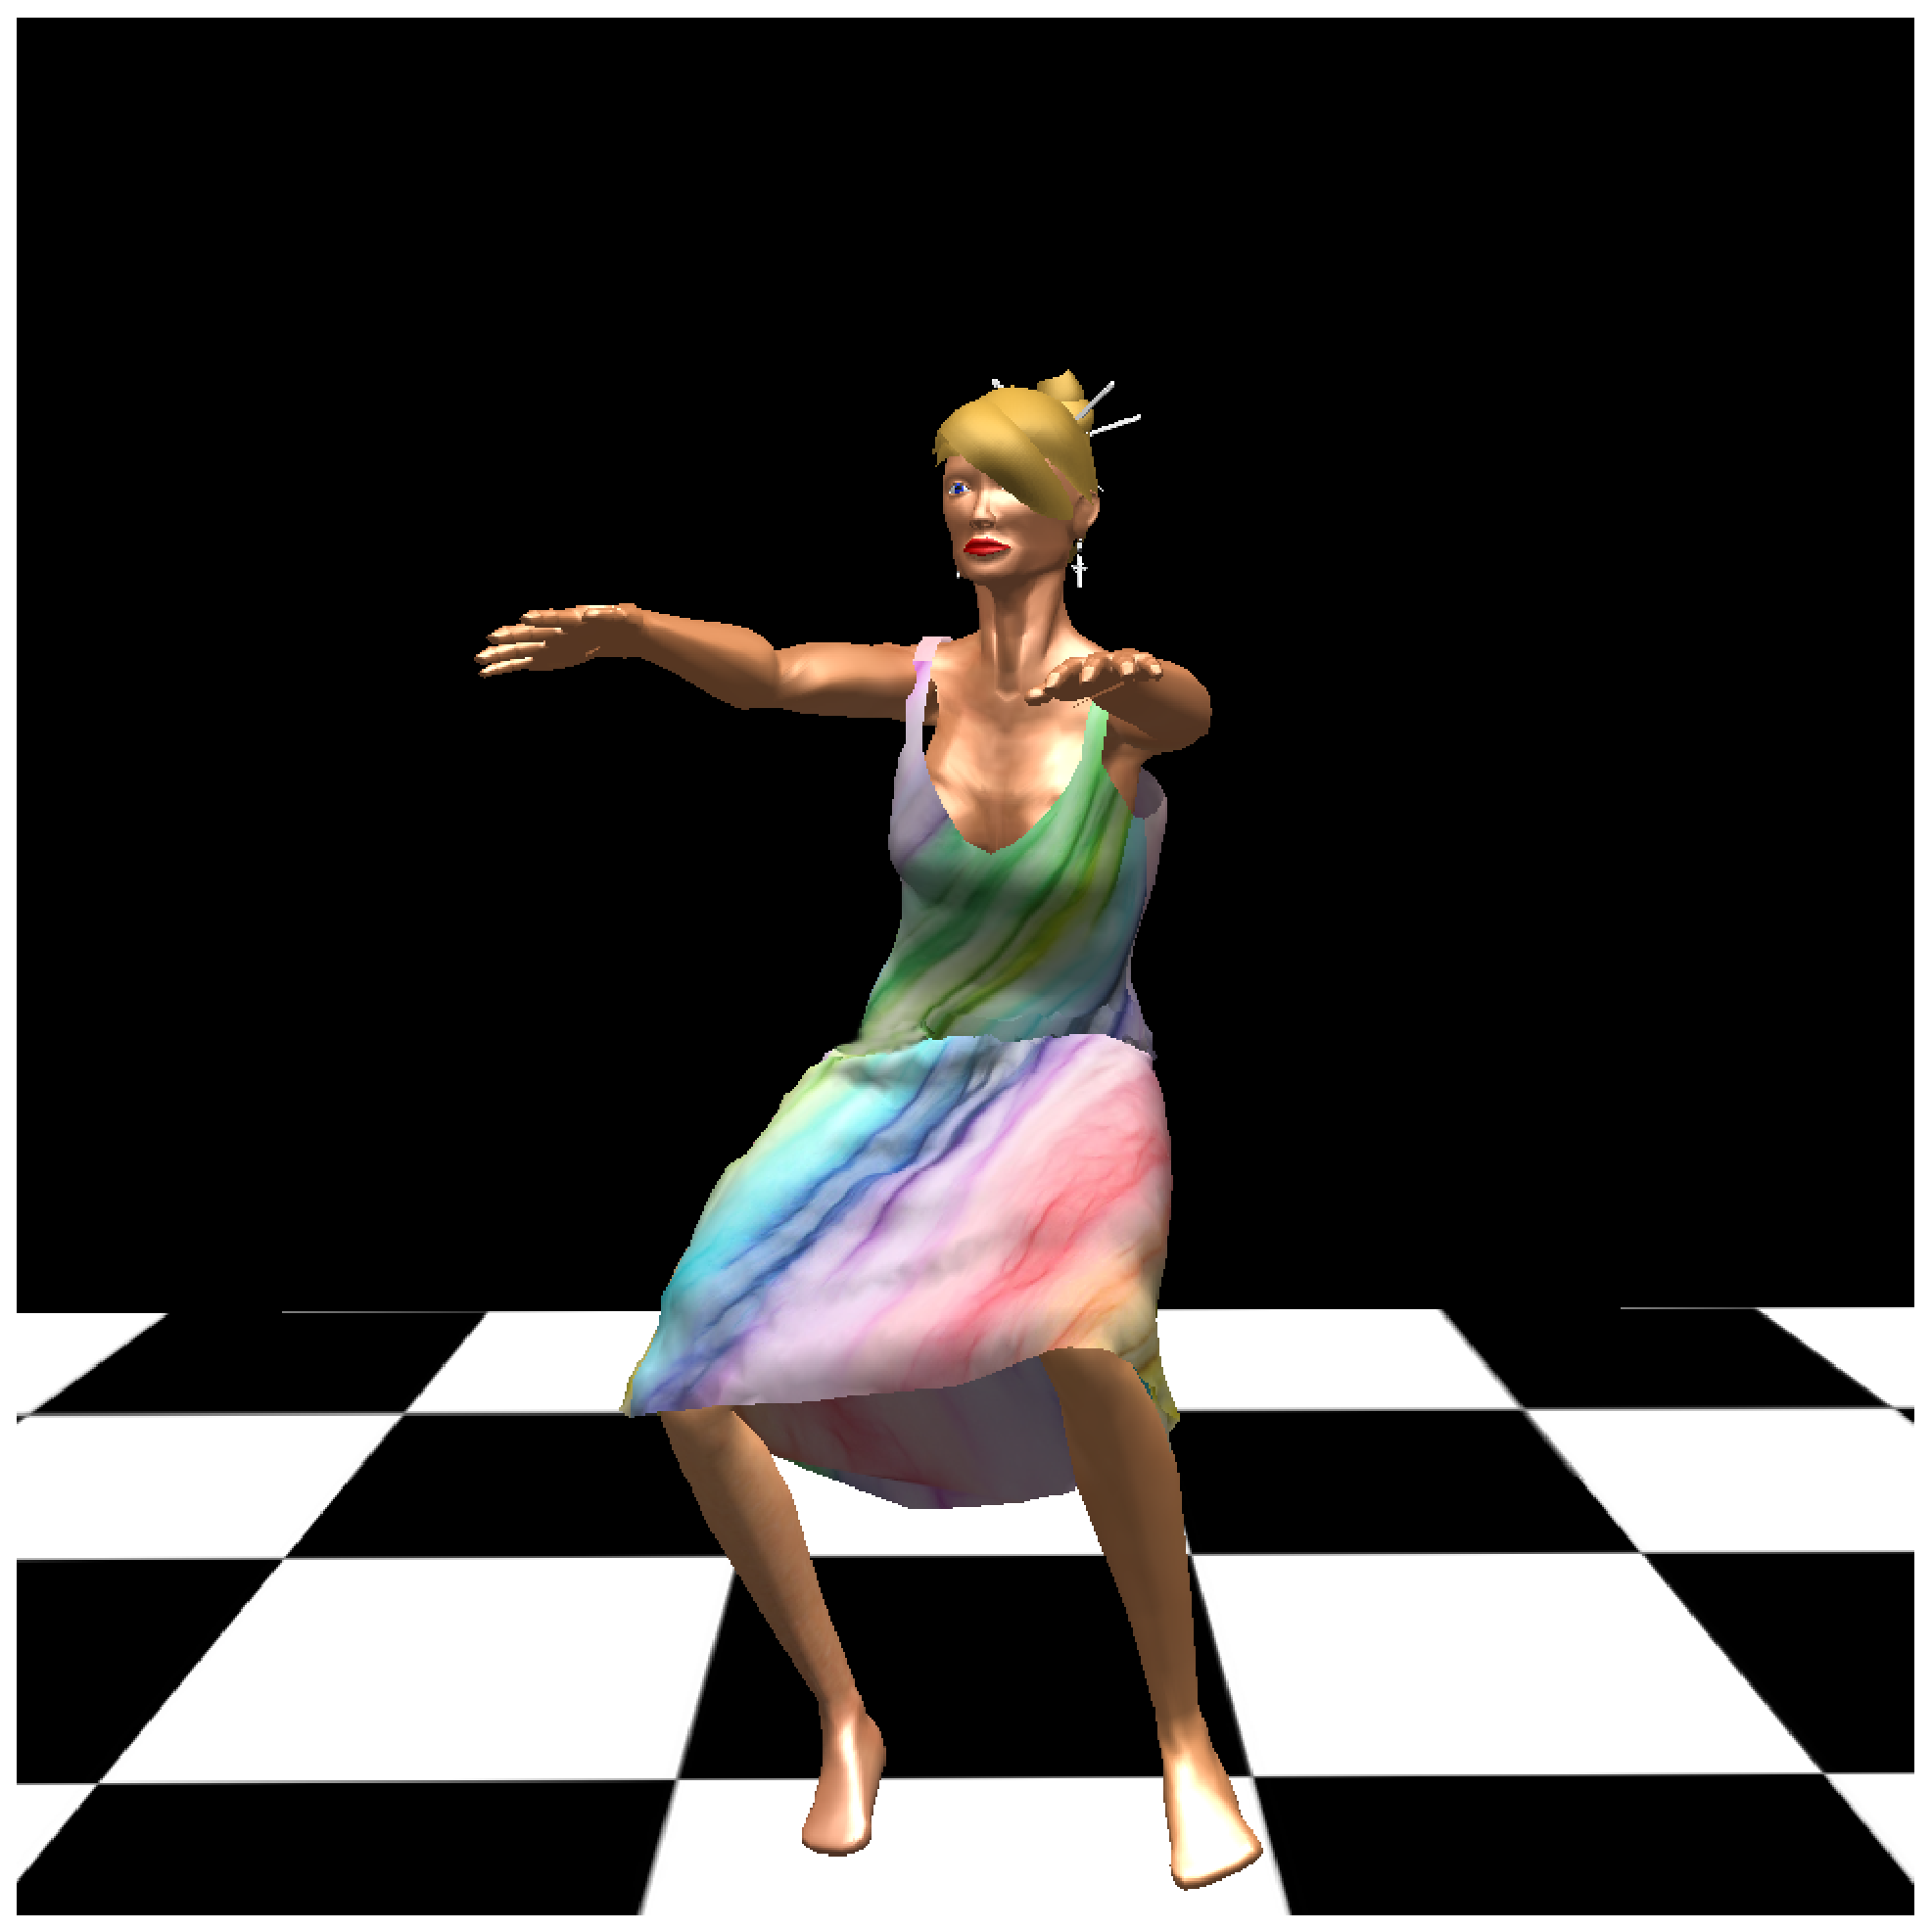
\includegraphics[width=0.250\textwidth]{./figures/sundress3.eps}
	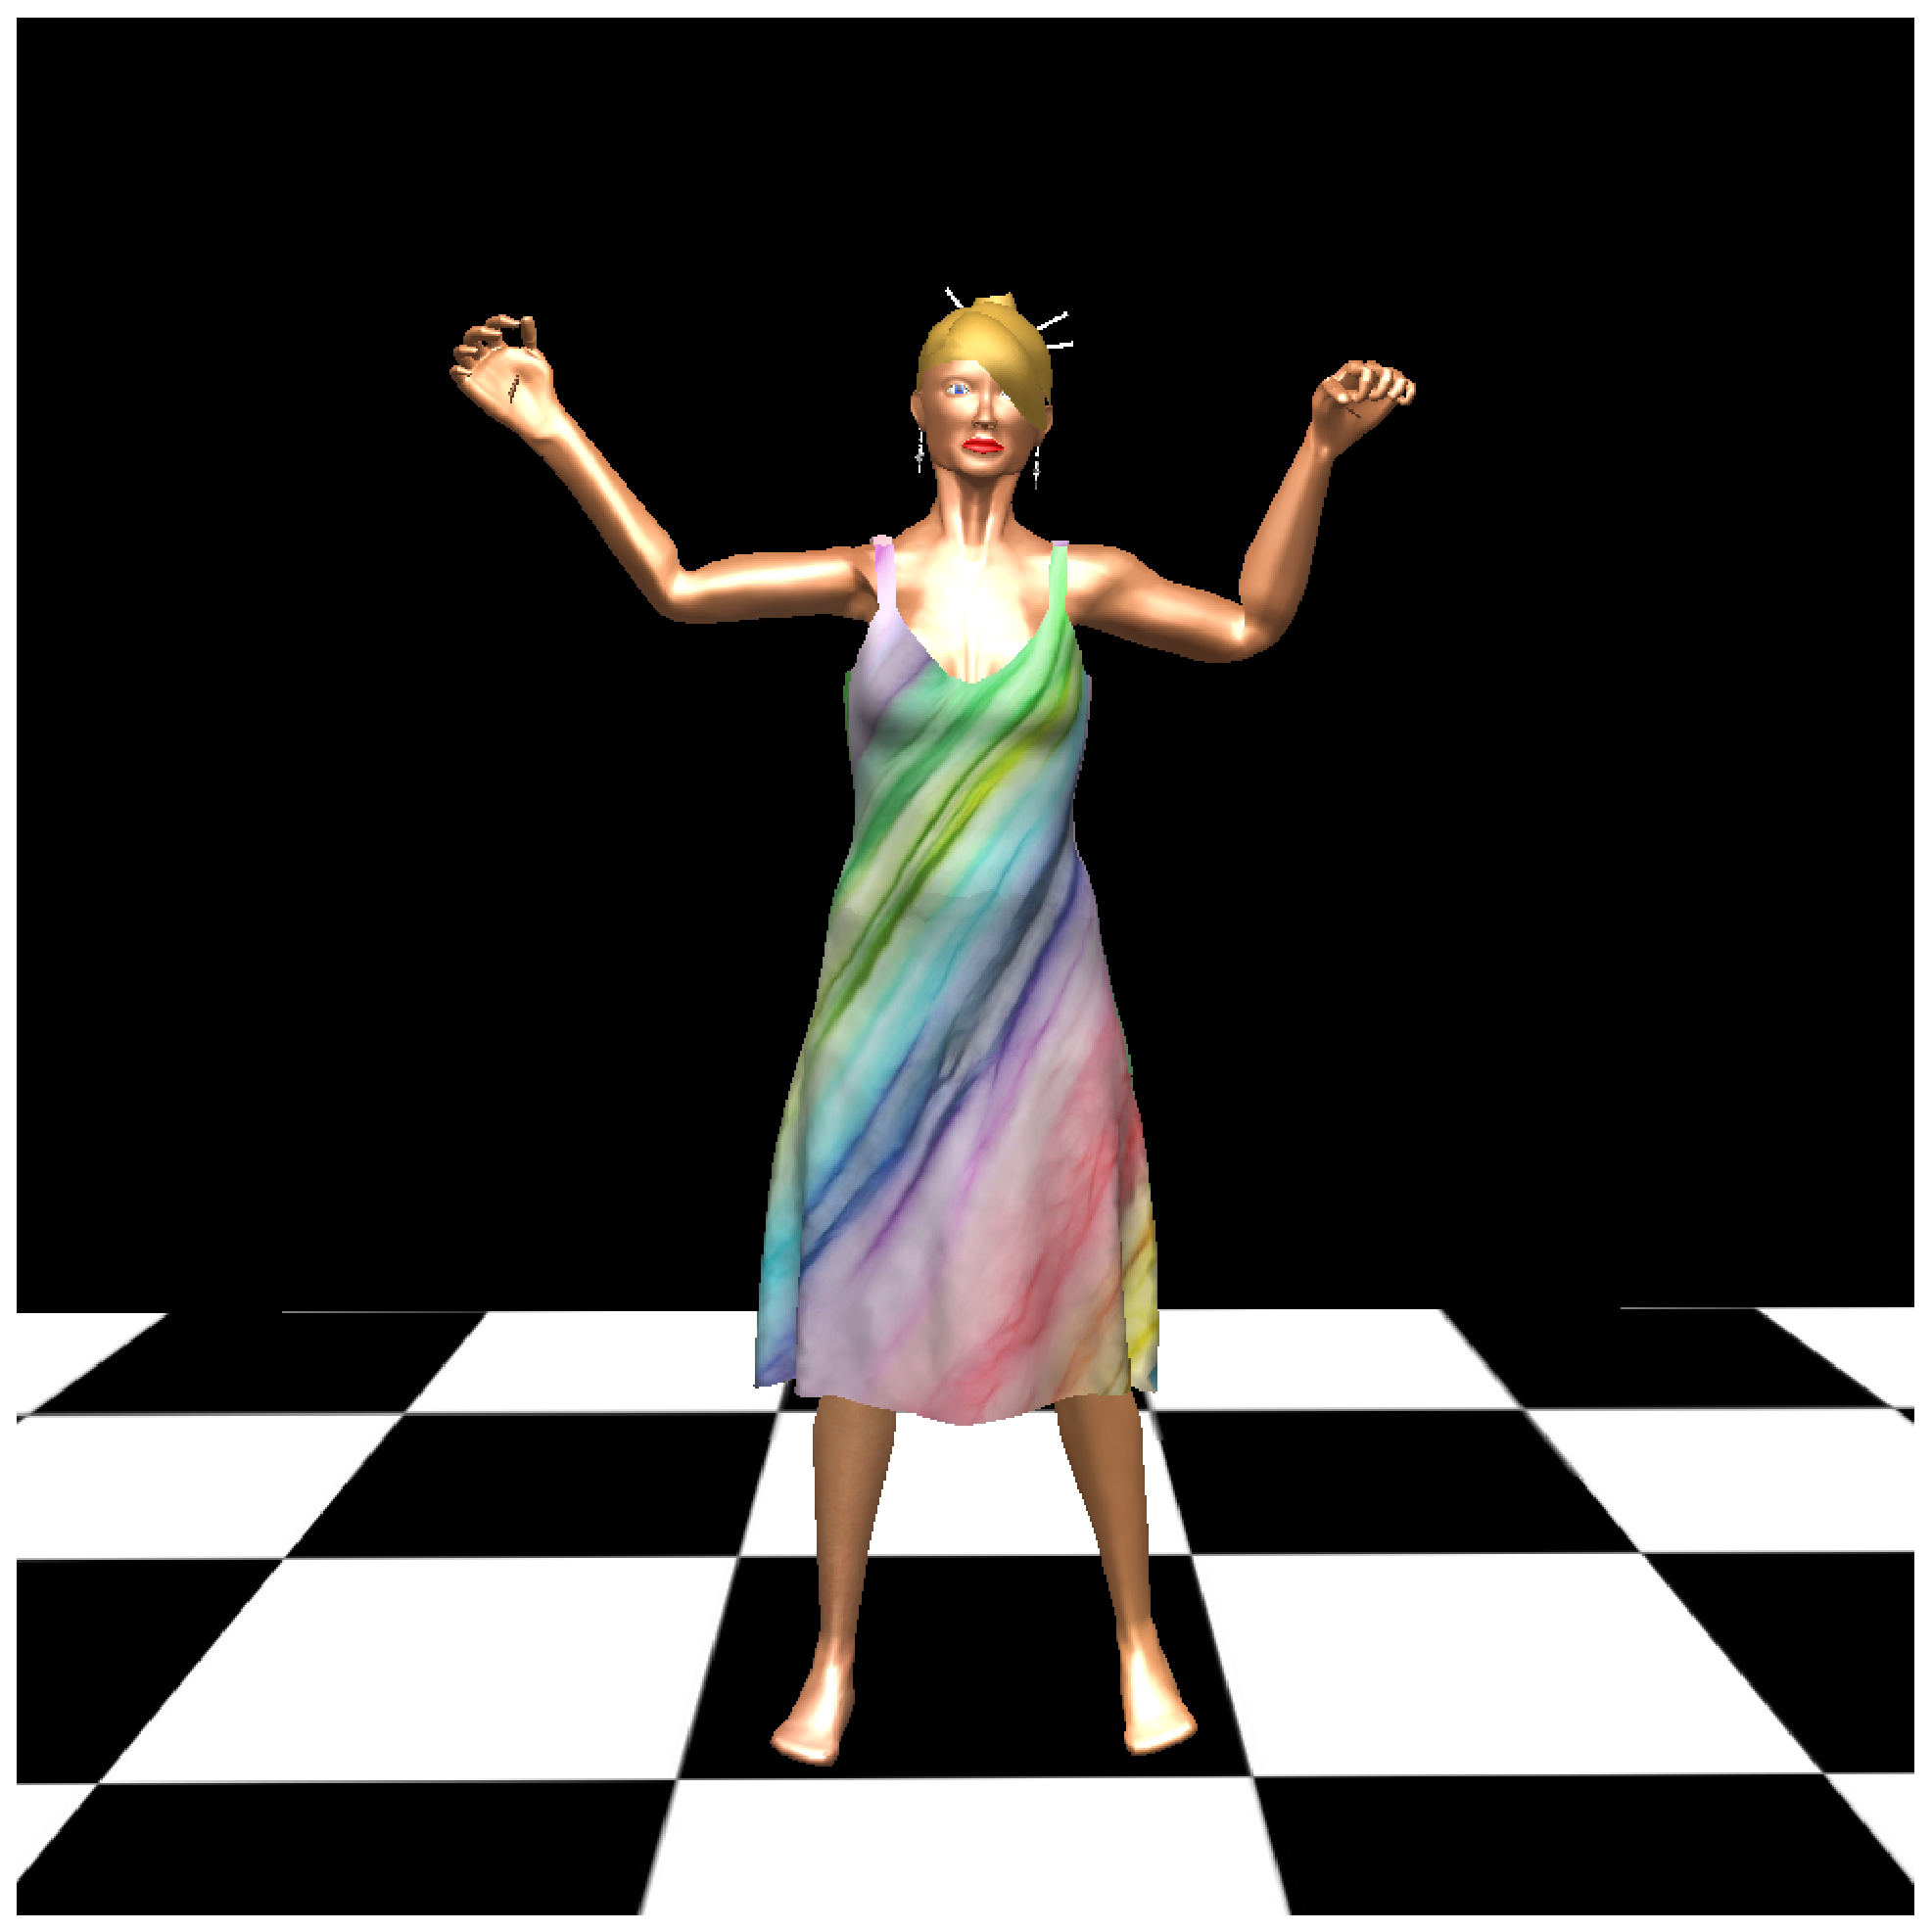
\includegraphics[width=0.250\textwidth]{./figures/sundress4.eps}
	}
	\centerline{(a)}
	\centerline{\ }
	\centerline{
	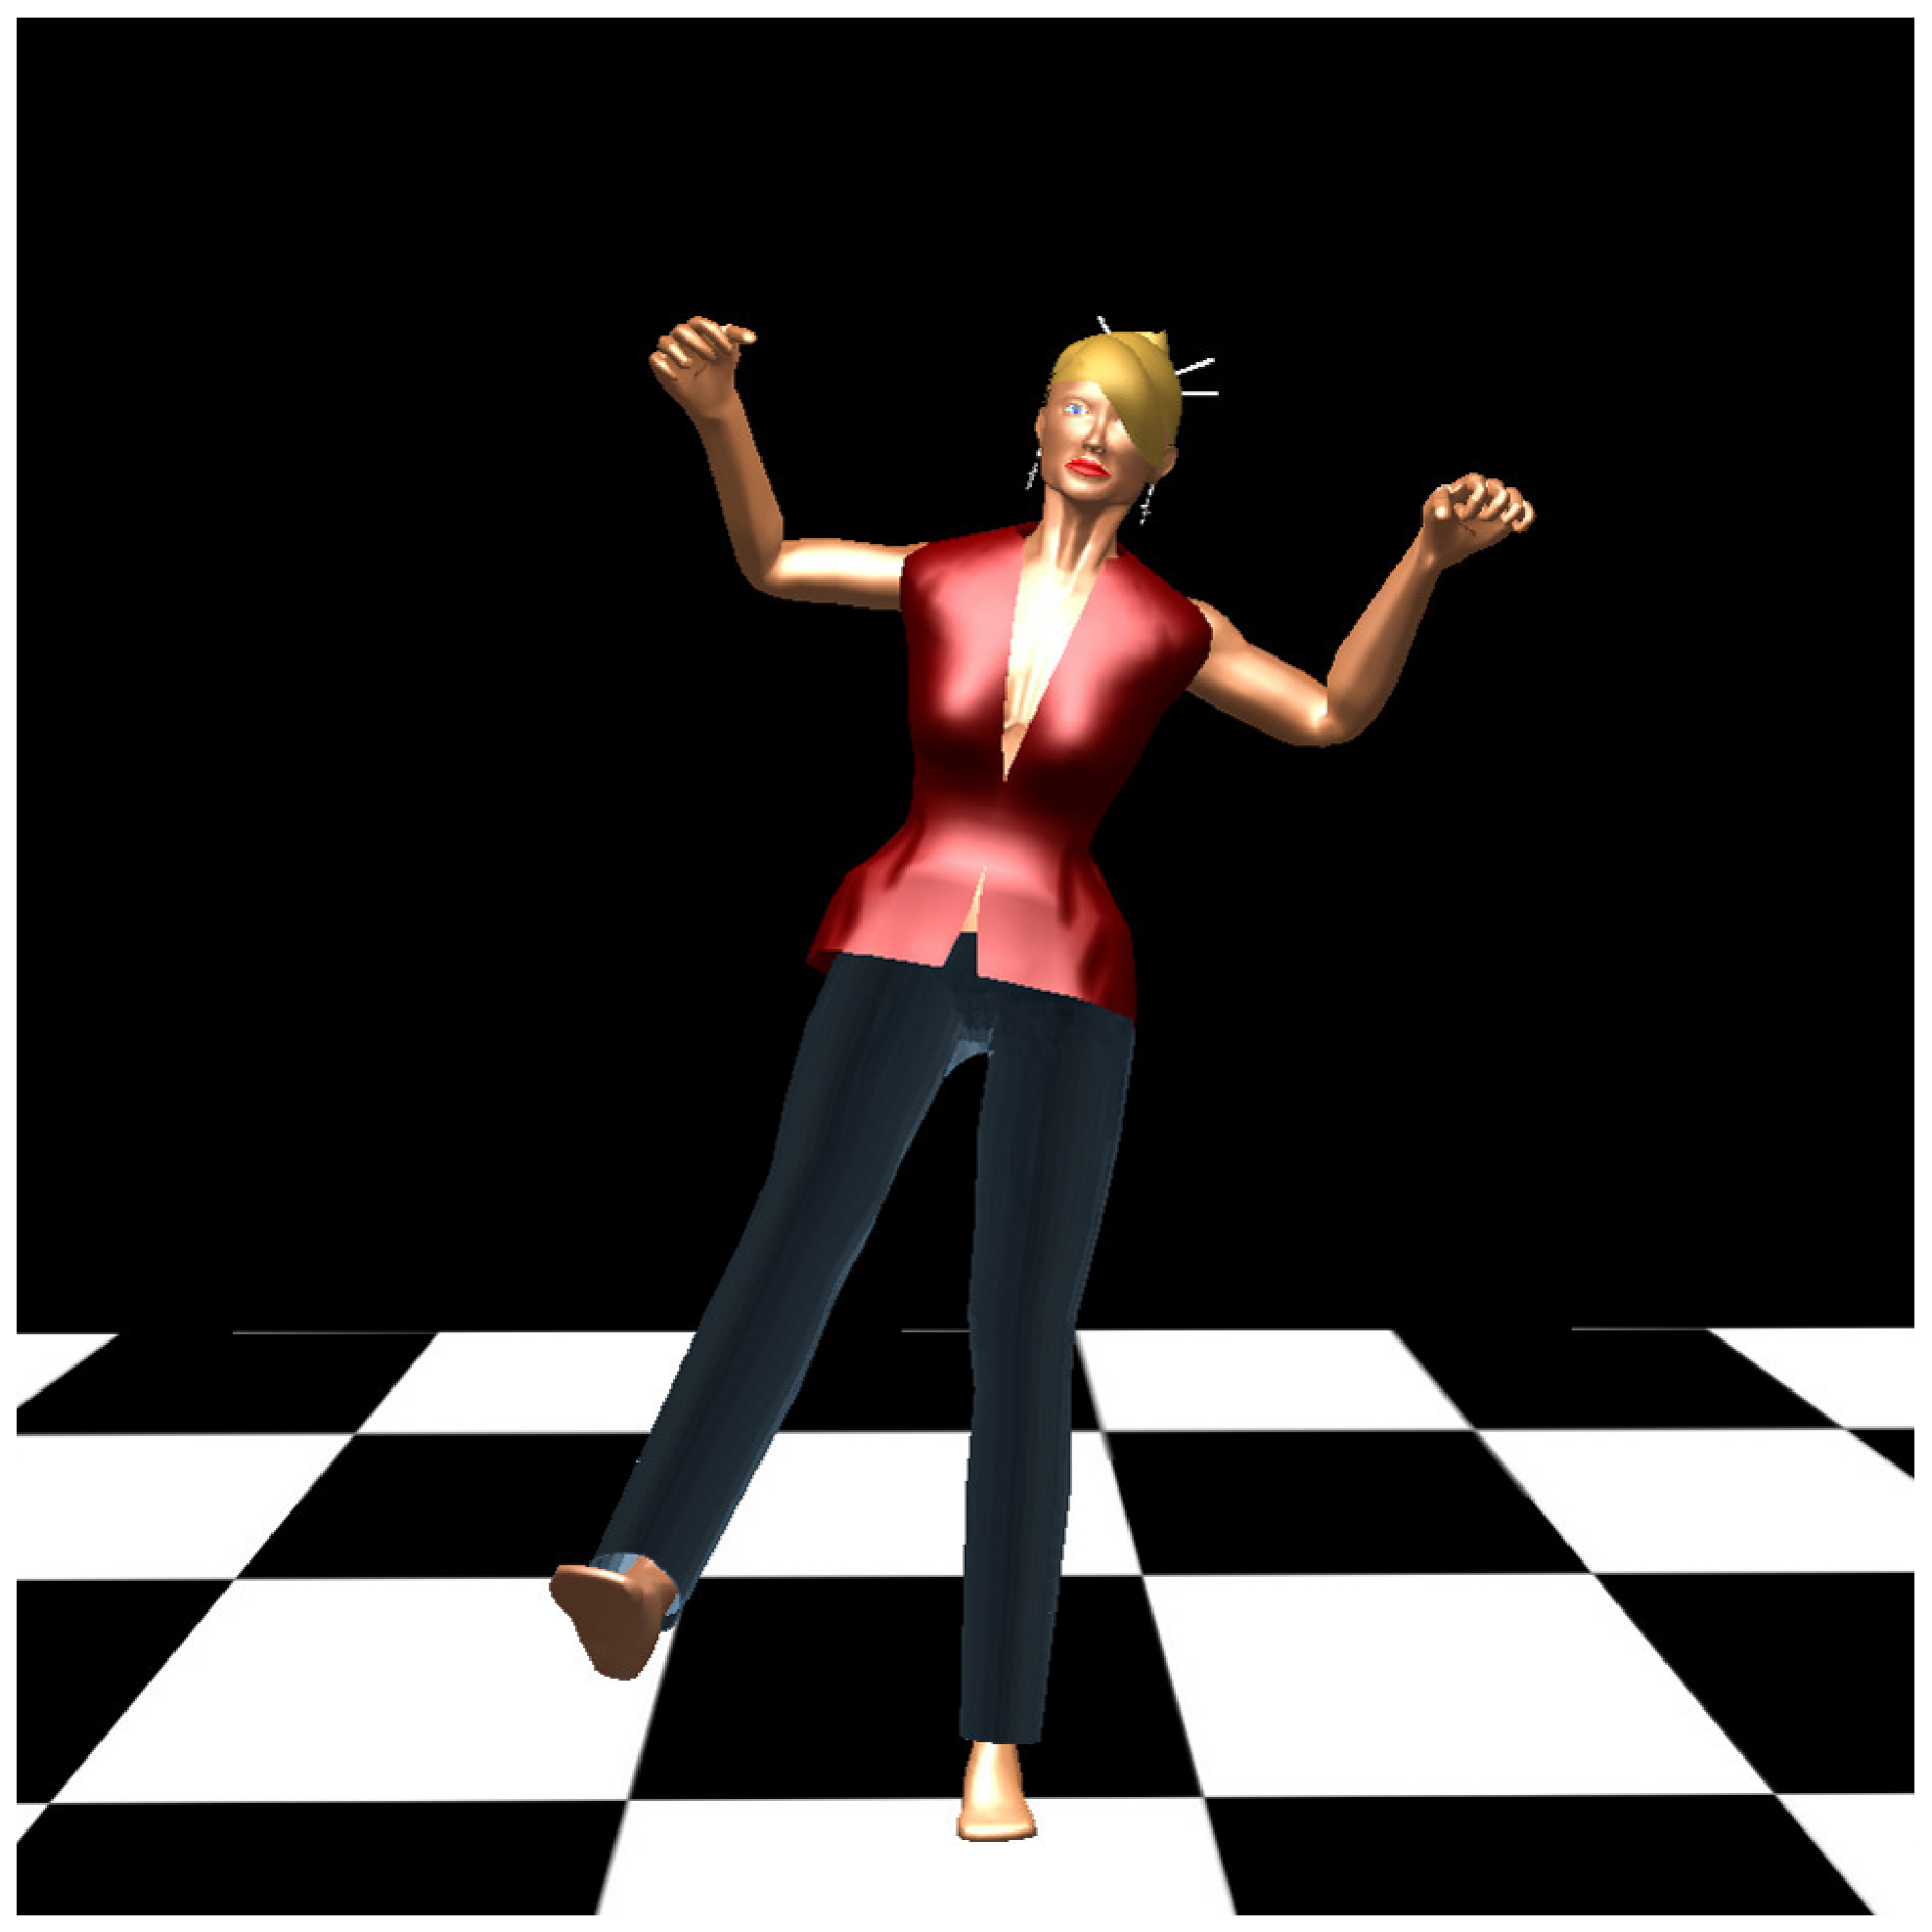
\includegraphics[width=0.250\textwidth]{./figures/jeans-1.eps}
	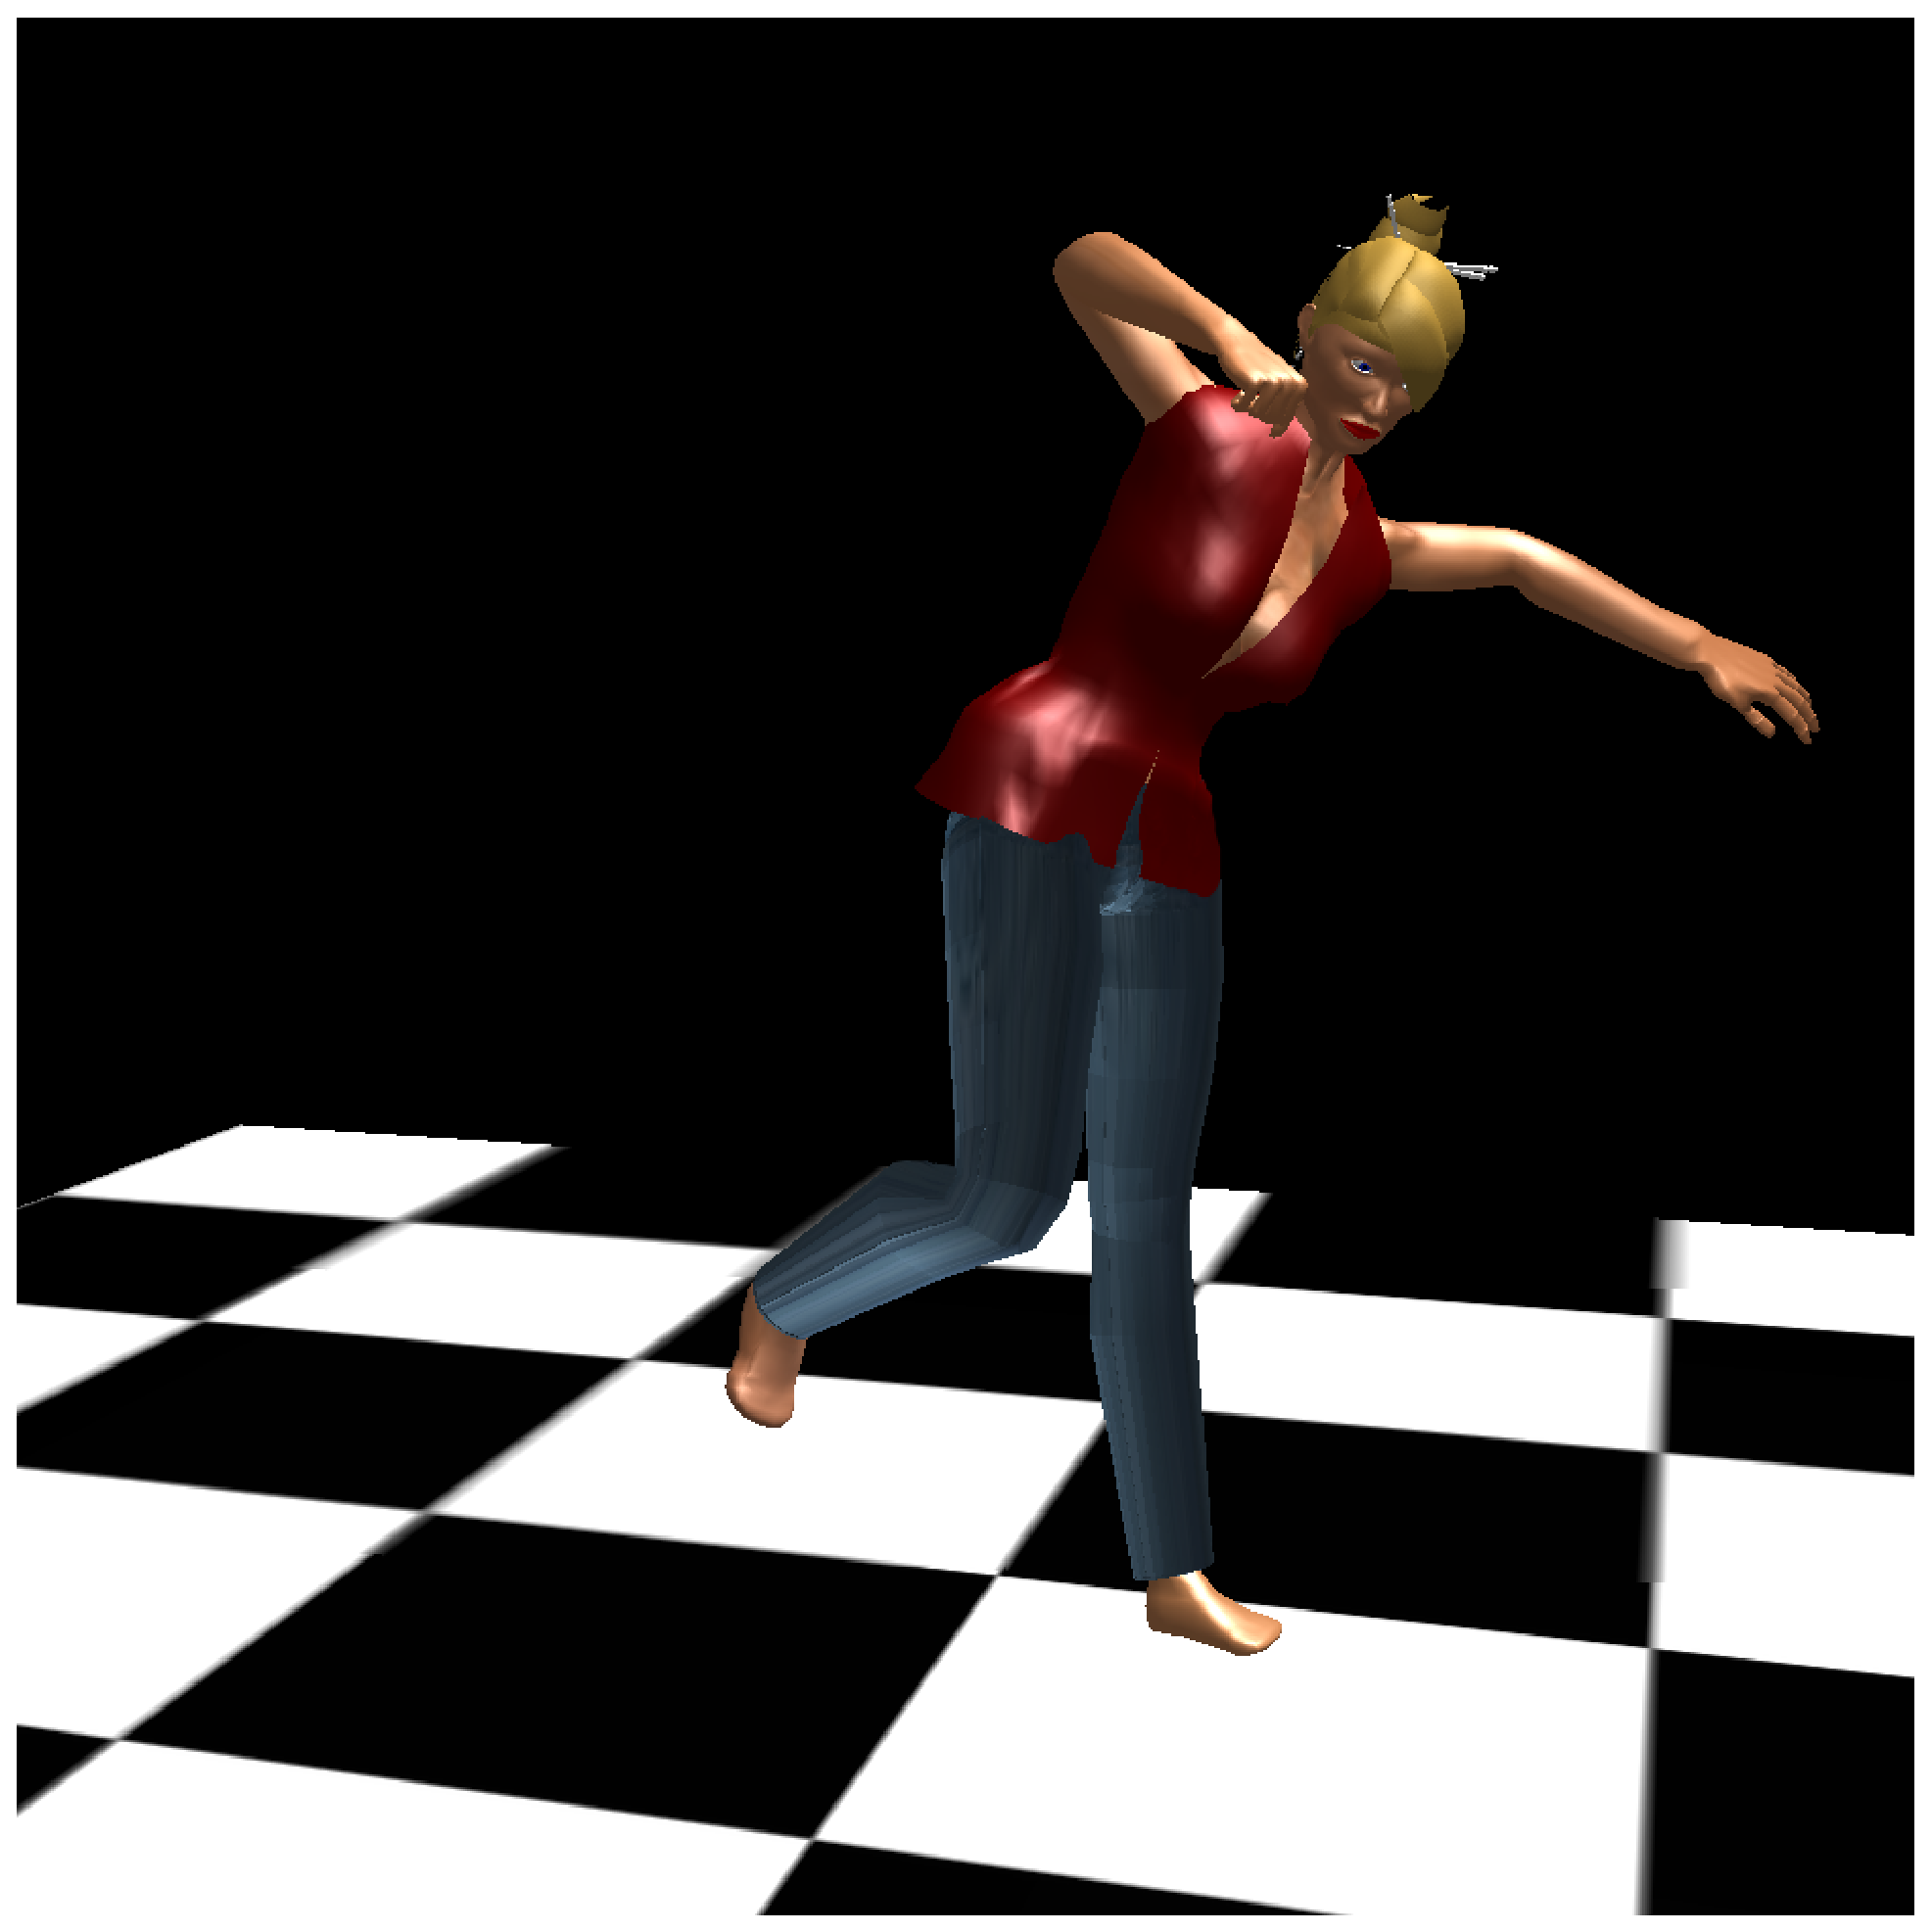
\includegraphics[width=0.250\textwidth]{./figures/jeans-2.eps}
	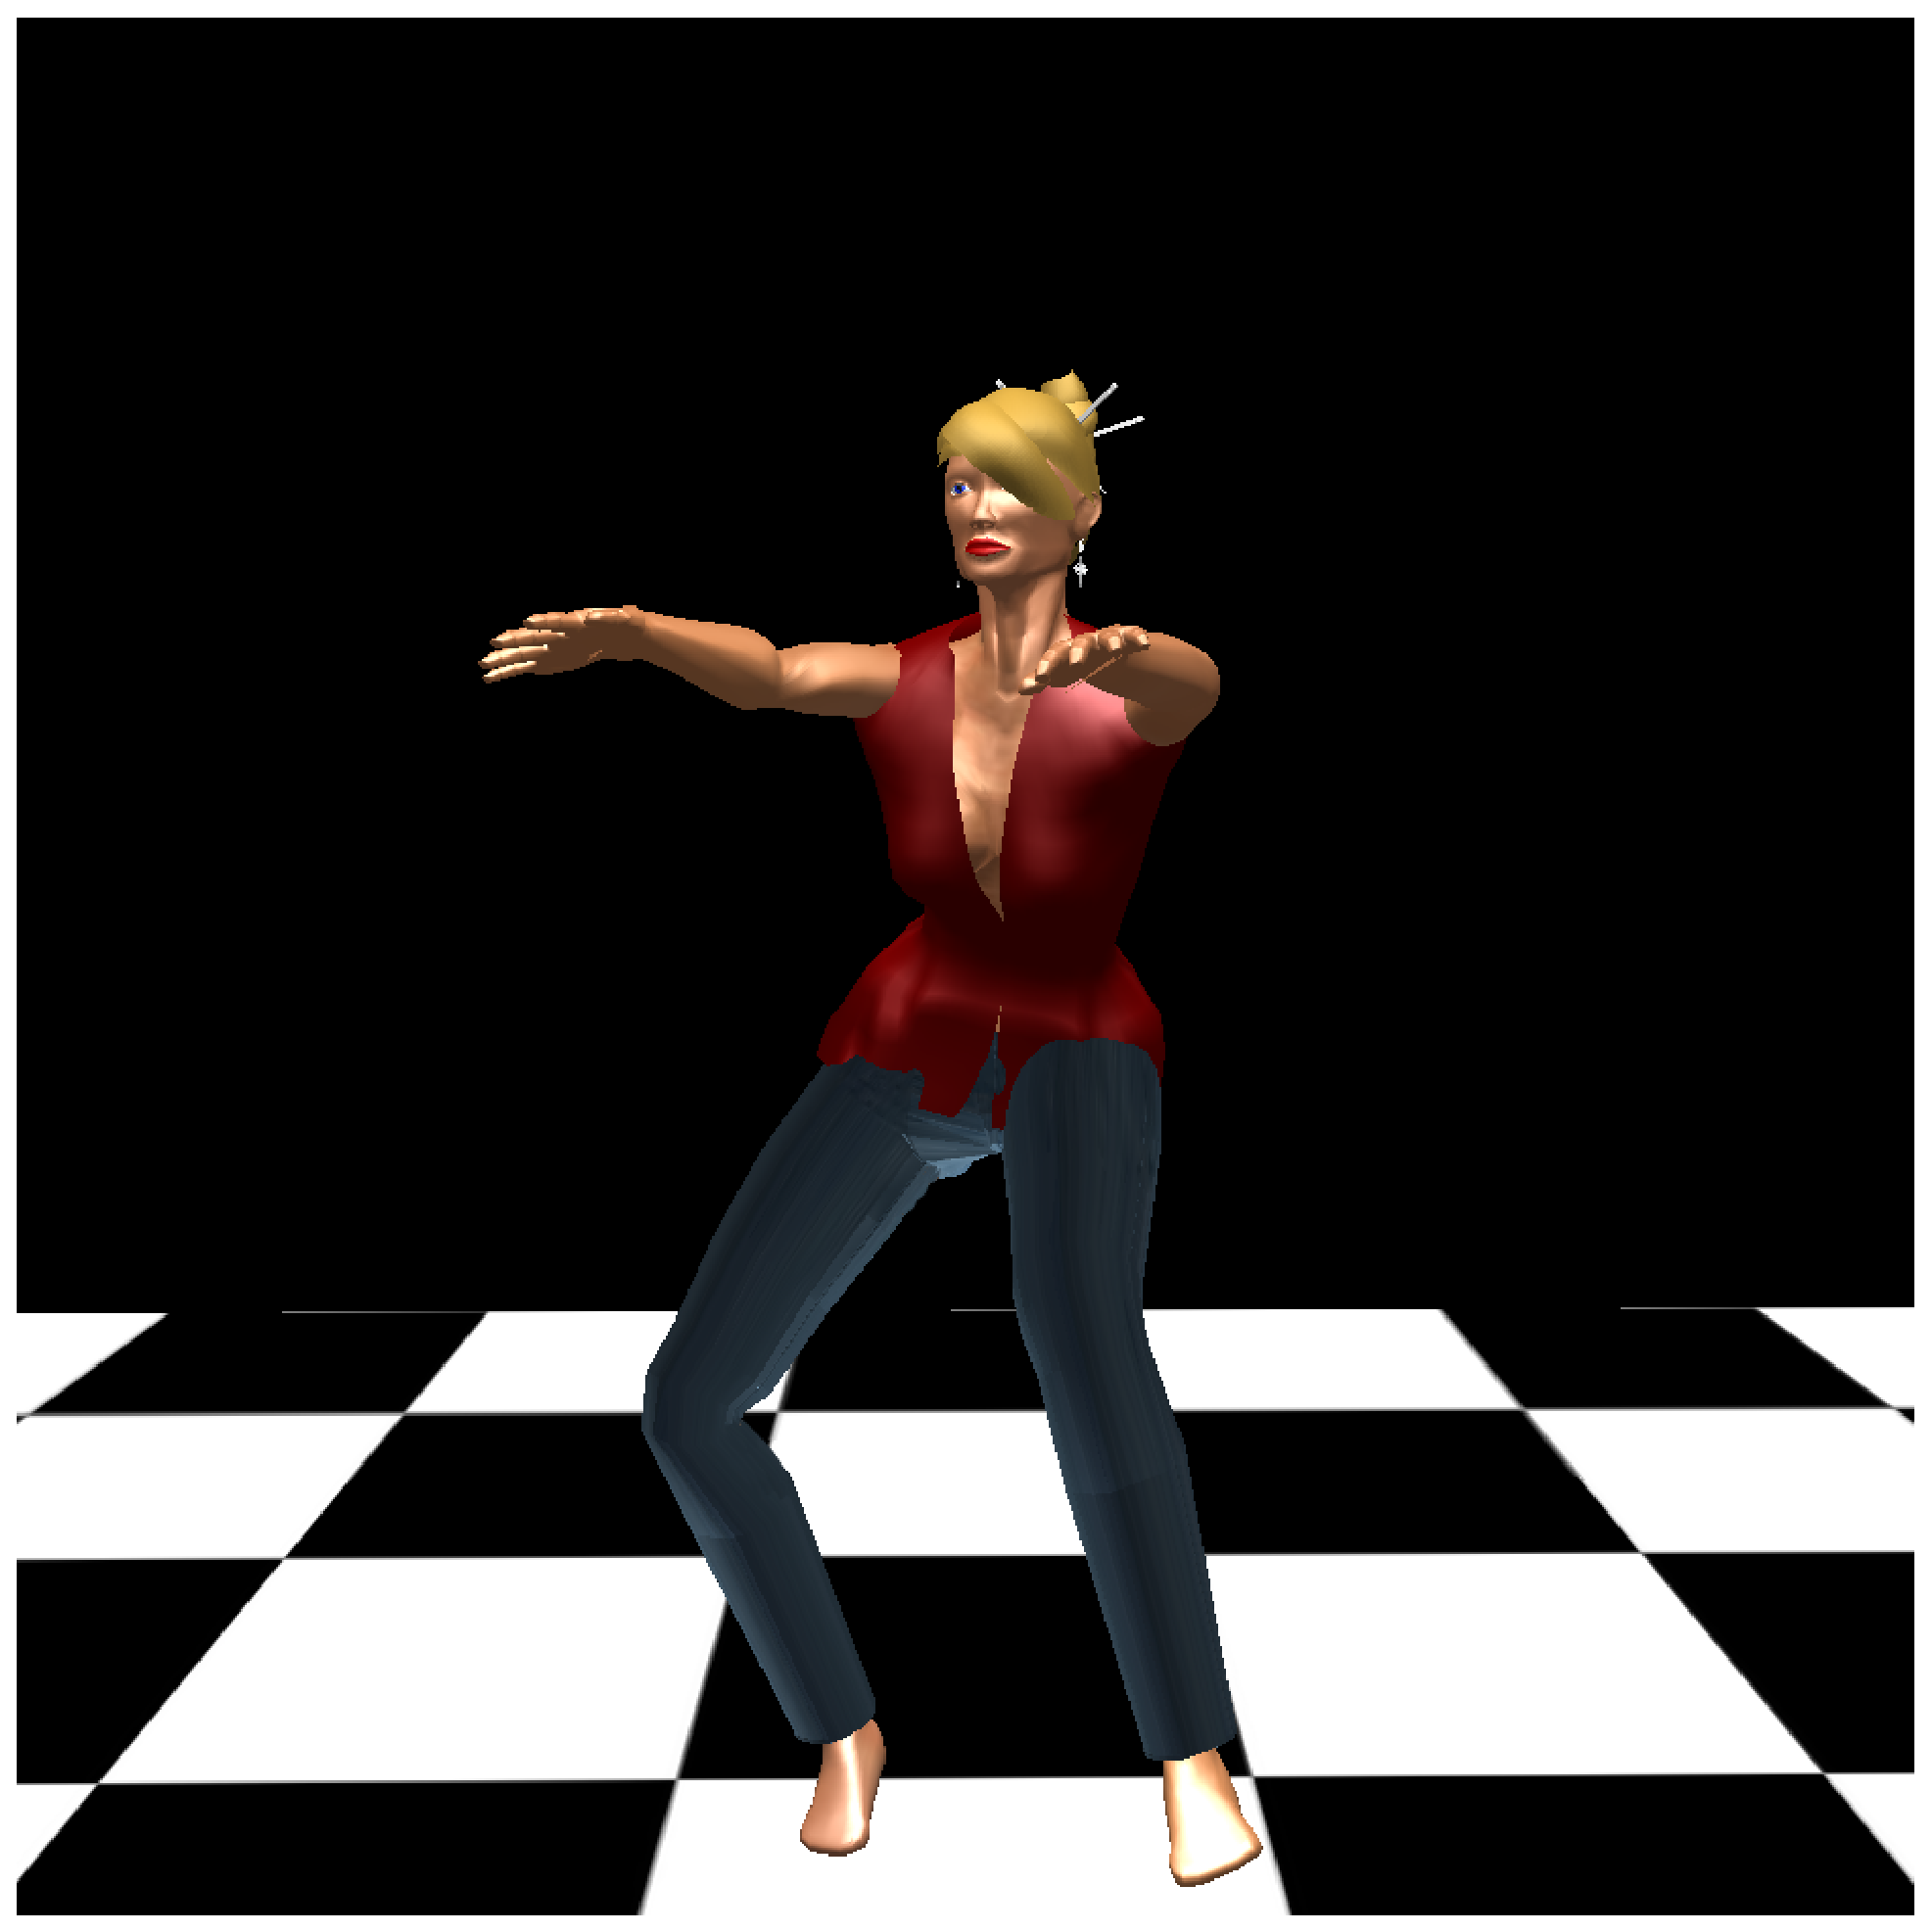
\includegraphics[width=0.250\textwidth]{./figures/jeans-3.eps}
	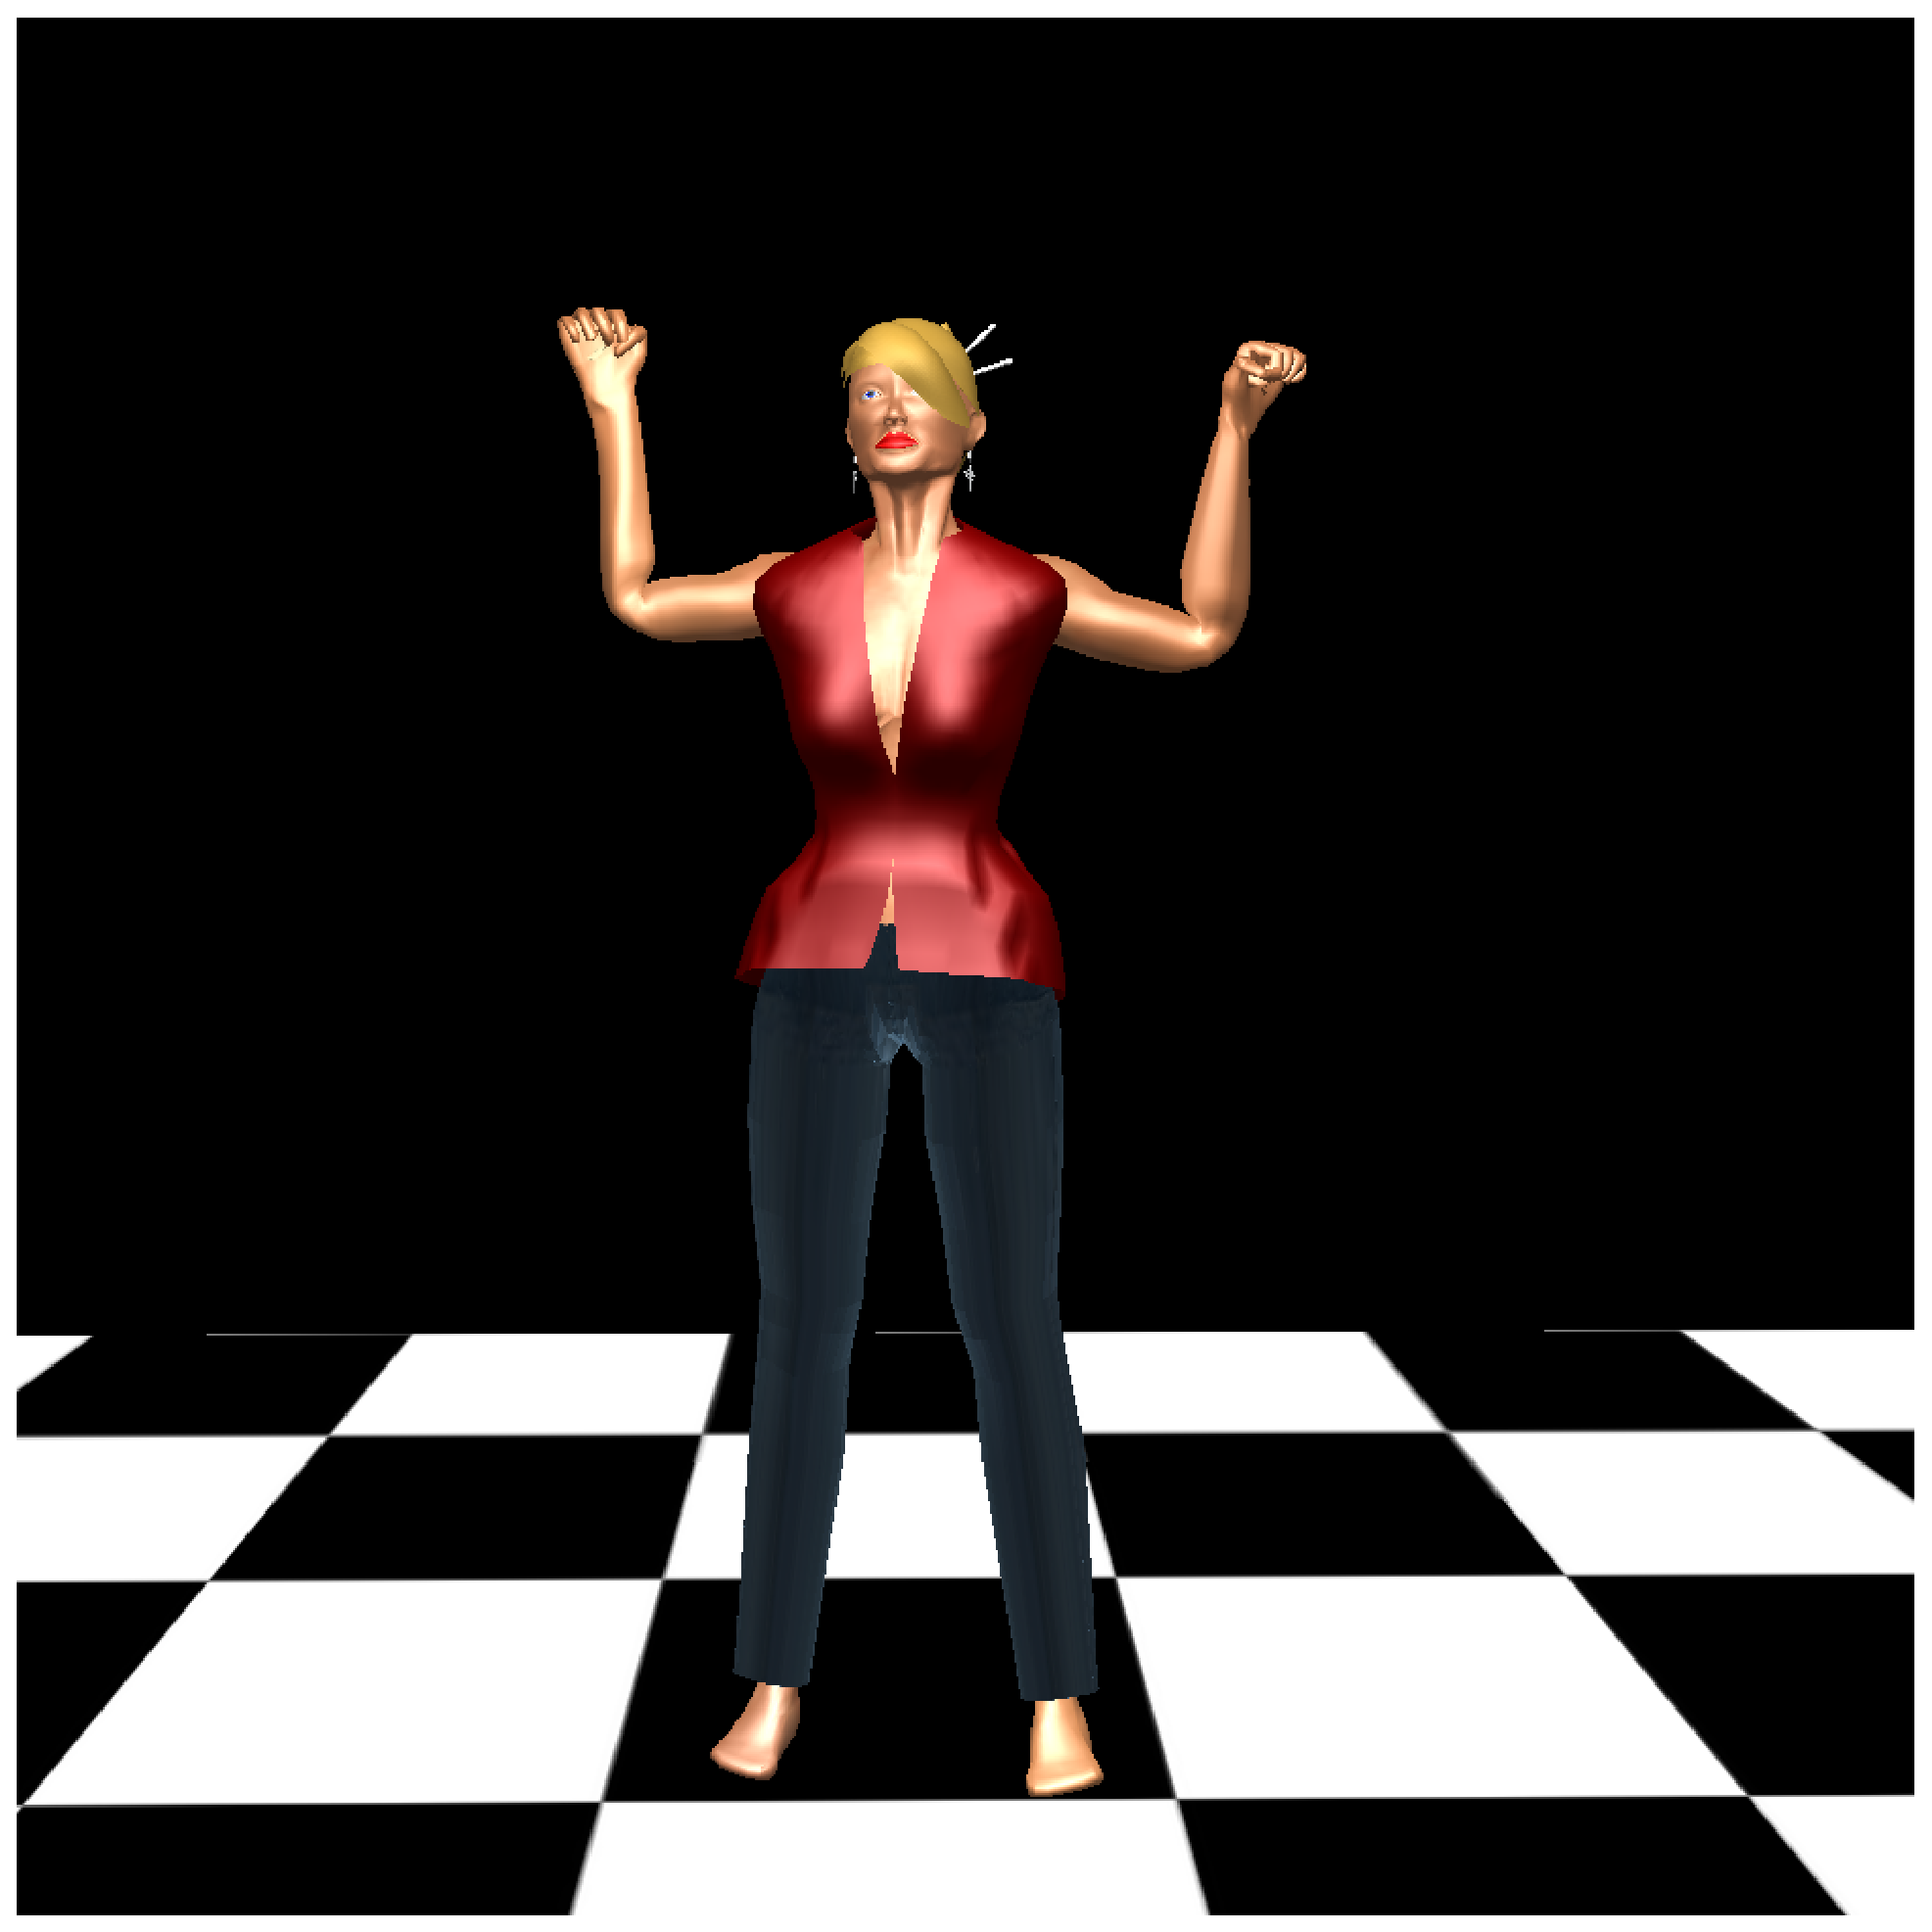
\includegraphics[width=0.250\textwidth]{./figures/jeans-4.eps}
	}
	\centerline{(b)}
	\centerline{\ }
	\centerline{
	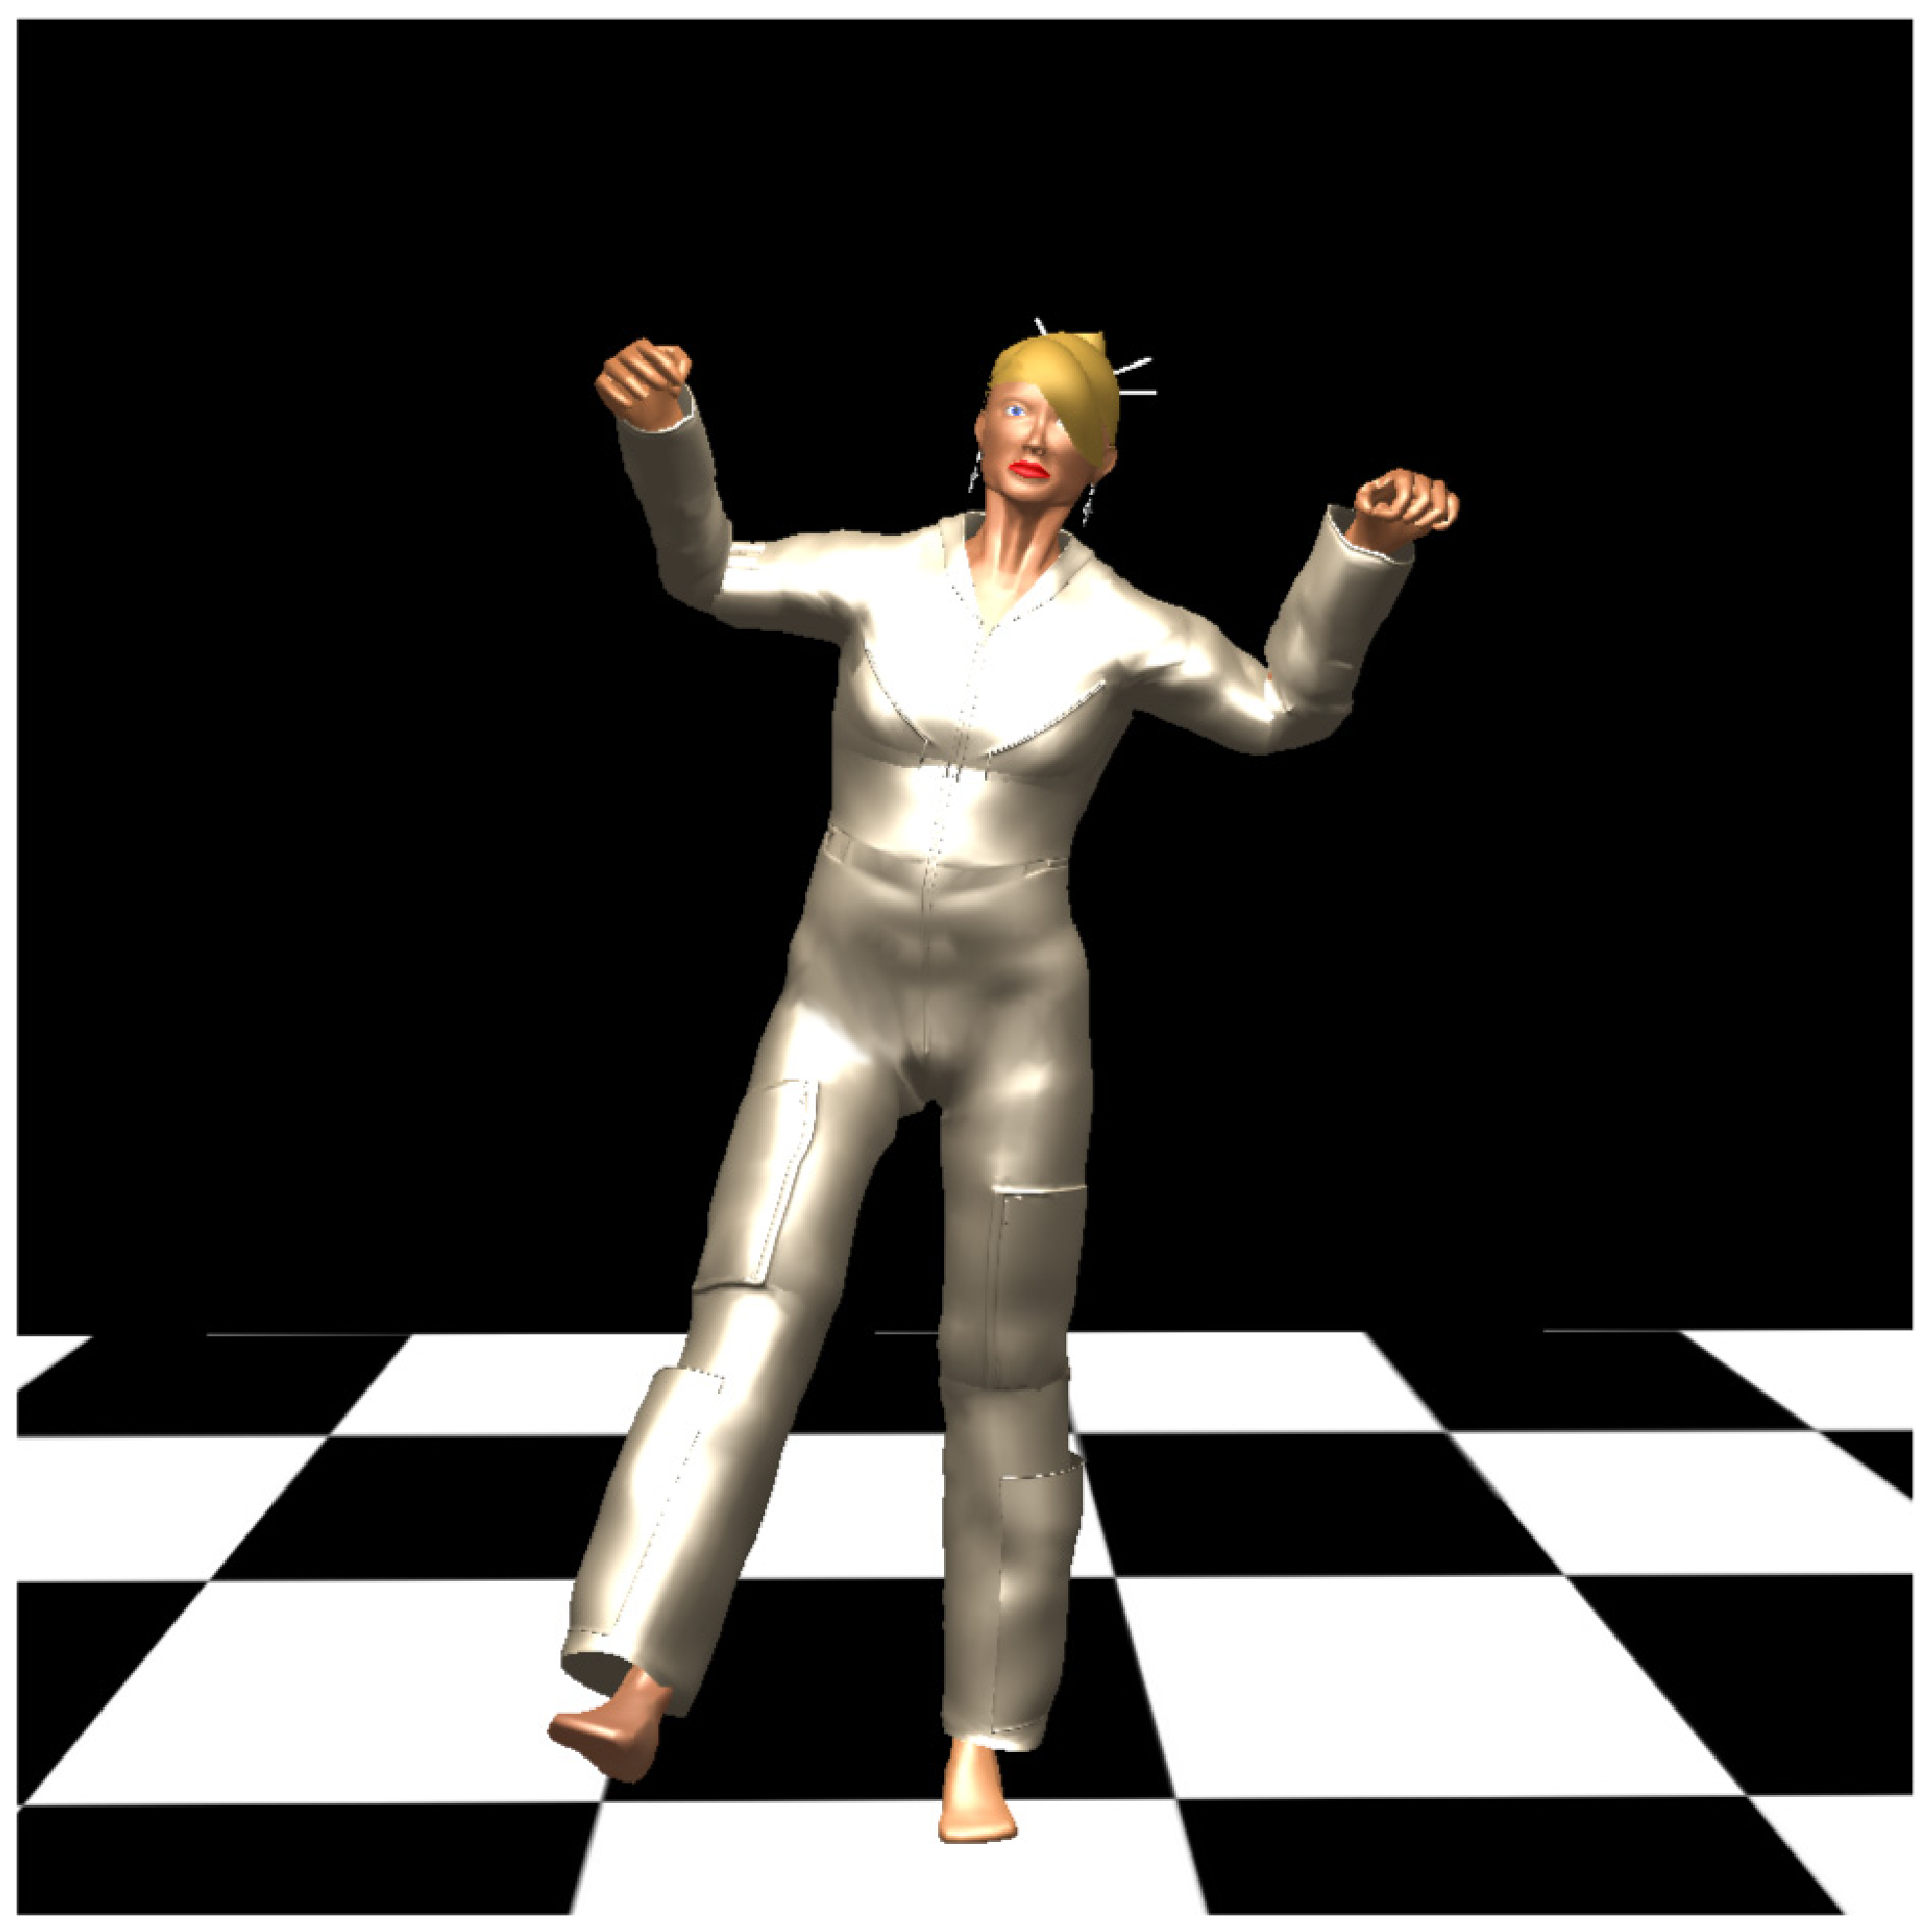
\includegraphics[width=0.250\textwidth]{./figures/flightsuit-1.eps}
	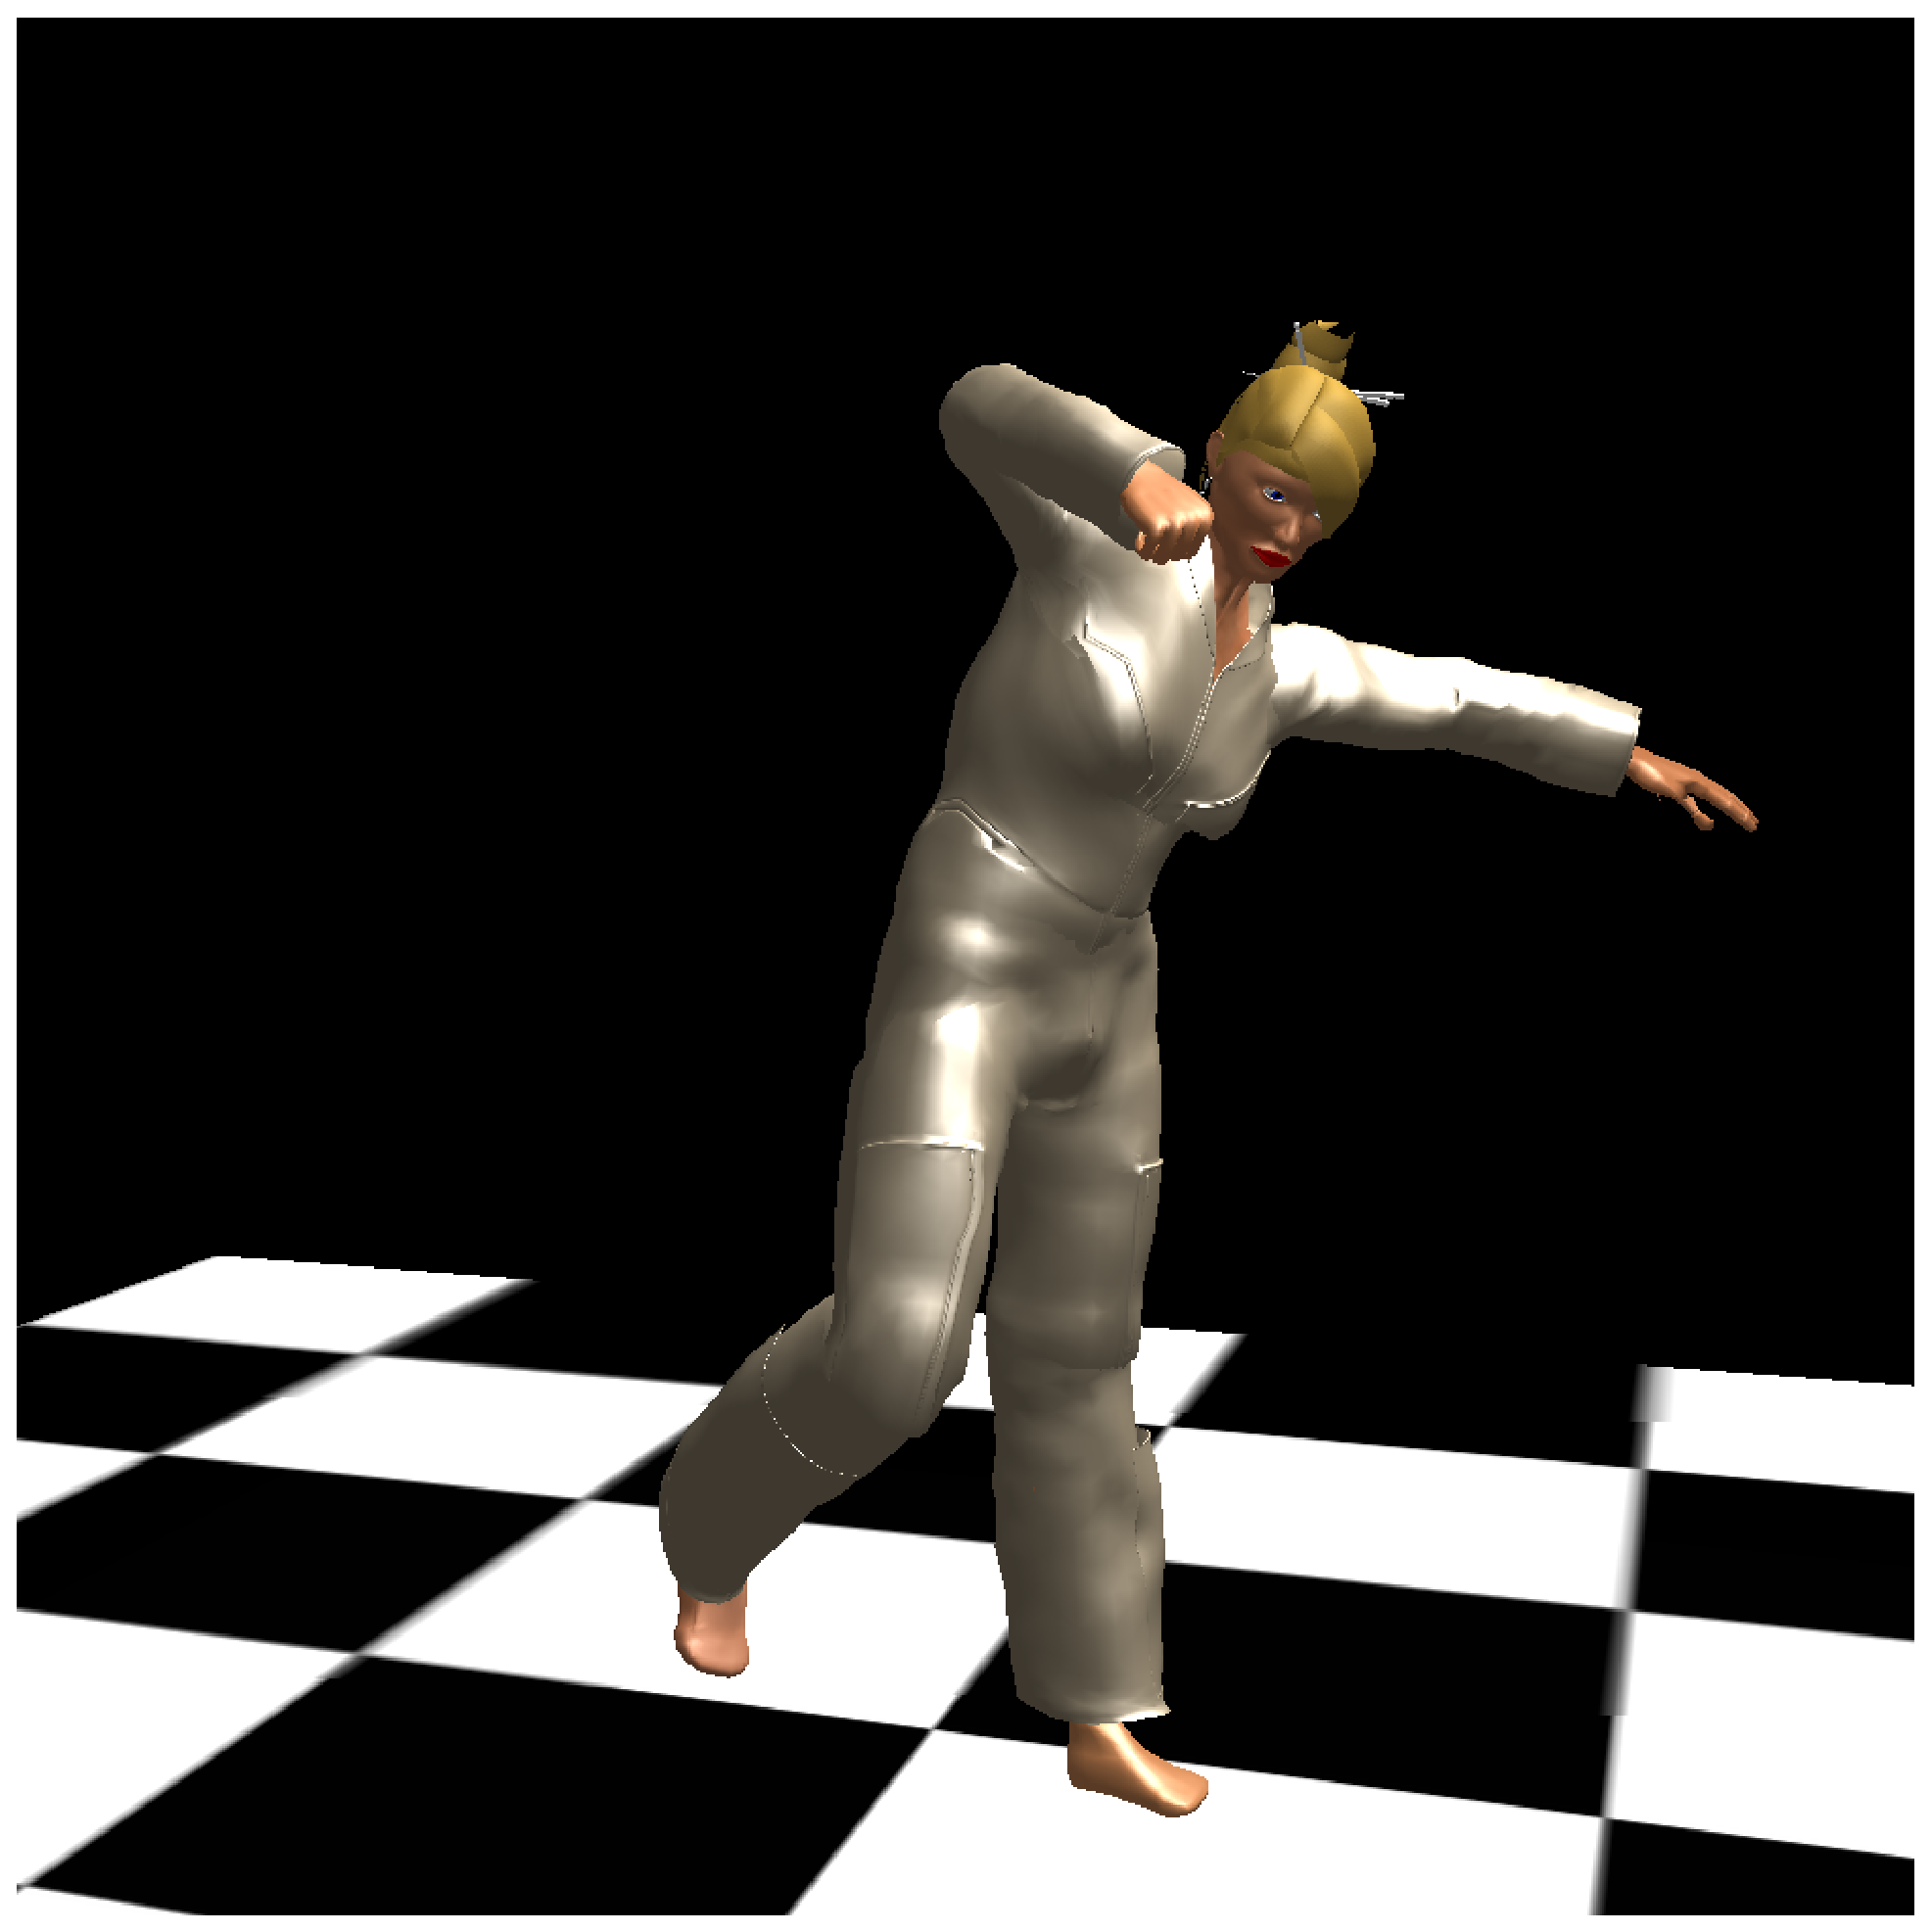
\includegraphics[width=0.250\textwidth]{./figures/flightsuit-2.eps}
	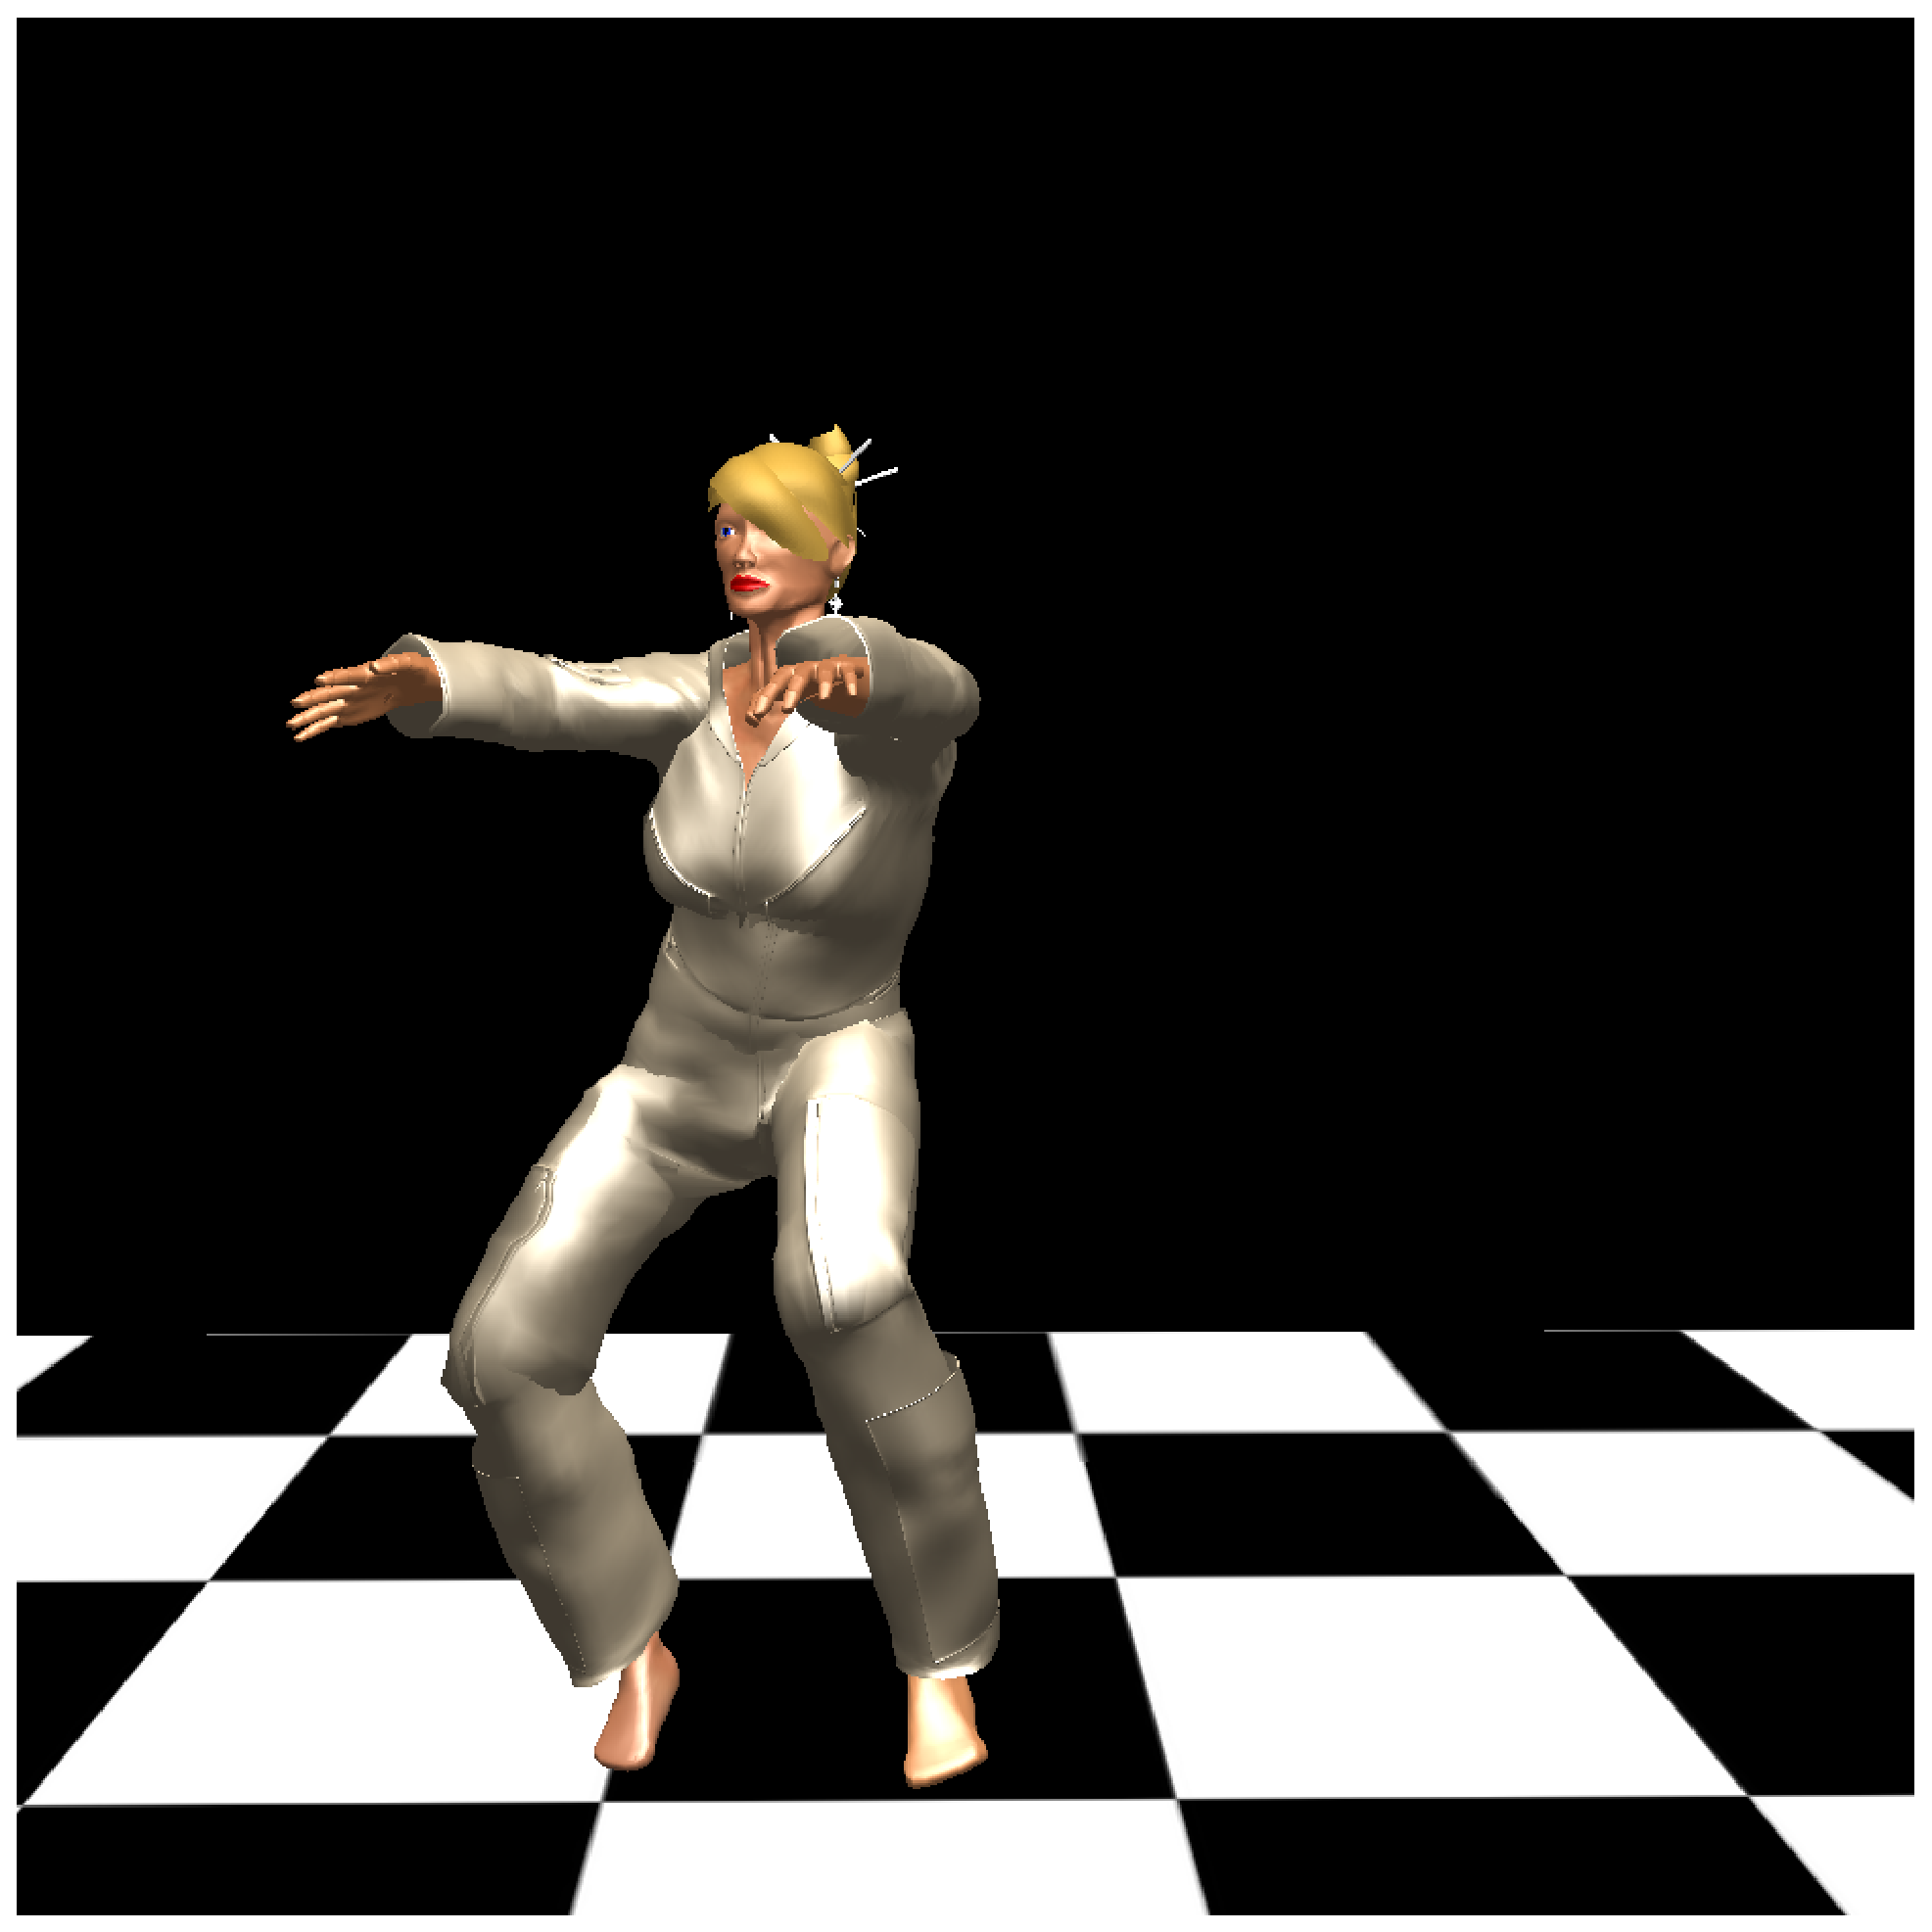
\includegraphics[width=0.250\textwidth]{./figures/flightsuit-3.eps}
	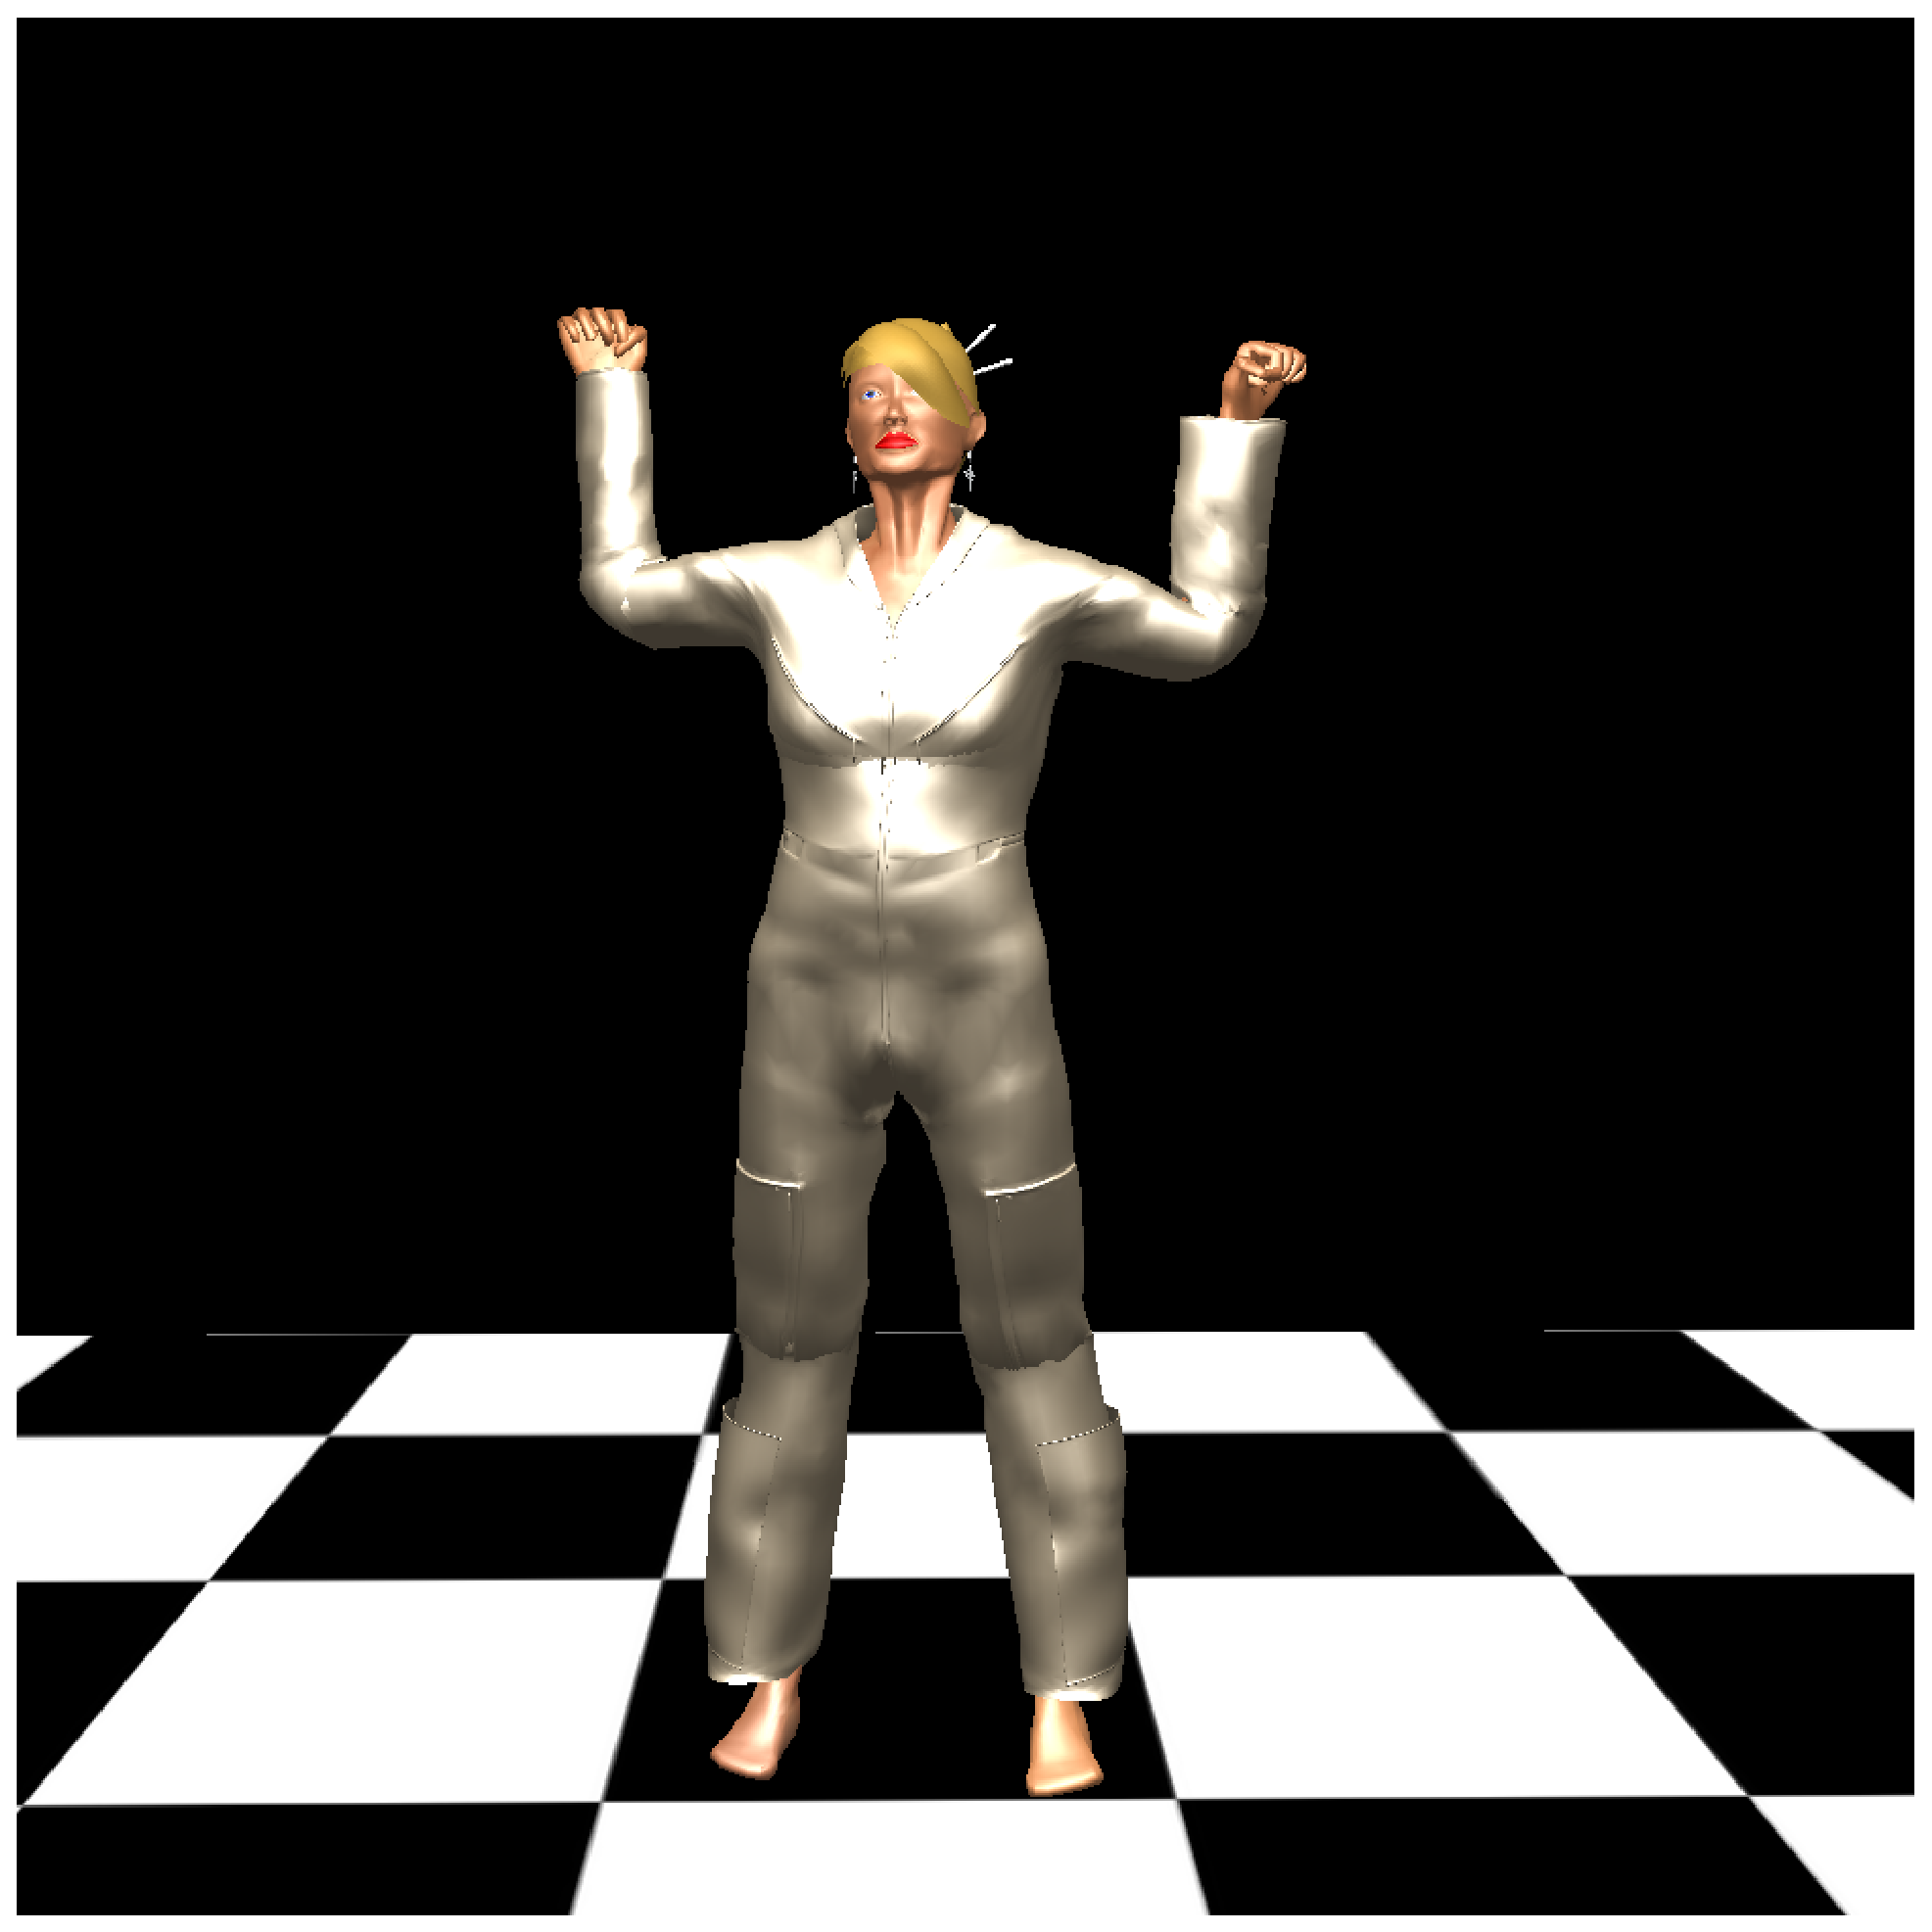
\includegraphics[width=0.250\textwidth]{./figures/flightsuit-4.eps}
	}
	\centerline{(c)}
	\caption{Examples of different garments on a model with different postures: (a) sun dress, (b) jeans and vest, and 
	(c) flight suit.}
	\label{fig:examples}
\end{figure}
